\documentclass{beamer}
\usepackage{graphicx}
\usepackage{tikz}
\usepackage{enumerate}
\usepackage{xstring}
\usetikzlibrary{fit,positioning}
\usetikzlibrary{shapes.geometric, arrows, positioning,shadows, calc, intersections}
\usepackage{animate} % For animation
\usepackage{pgfplots} % For plots
\usepackage{shellesc}
\usepackage{tcolorbox}
\usepackage{colortbl}
\usepackage{xcolor}
\usepackage{colortbl}
\usepackage{graphicx}
\usepackage{adjustbox}
\usepackage{array}
\usepackage{amsmath}
\usepackage{listings}
\pgfplotsset{compat=1.18}
\maxdeadcycles=200
\usetikzlibrary{matrix}
\usetikzlibrary{shapes.geometric, arrows}


\usetheme{Madrid}
\usecolortheme{orchid}

\definecolor{myorange}{rgb}{0.85, 0.49, 0.13}
\definecolor{myblue}{rgb}{0.15, 0.65, 0.90}
\definecolor{mygreen}{rgb}{0.19, 0.82, 0.28}
\definecolor{myred}{rgb}{0.85, 0.11, 0.11}


\title{Beamer Presentation for CSE200}
\subtitle{AutoEncoder}
\author{A2 Group 10}
\institute[CSE, BUET]{Department of CSE, BUET}



\begin{document}


% NABIHA TAHSEEN - 2105031


\begin{frame} 
    \maketitle
\end{frame}


% Slide: Describing a Person
\begin{frame}[t]{Describing a Person}
    \begin{center}
        \begin{tikzpicture}[
            person/.style={draw, fill=white, minimum size=1.5cm},
            label/.style={font=\large, align=left},
            feature/.style={font=\Large\color{black!70!black}, align=left},
            arrow/.style={->, thick, color=blue!50!black}
        ]
            % Person icon
            \node[person] (person) at (-2, 1.5) {\includegraphics[scale=0.14]{person.jpg}};
            
            % Features
            \node[feature] (hair) at (2, 2.5) {Hairstyle:  \color{red!100!red} Curly};
            \node[feature] (age) at (2, 1.5) {Age:  \color{red!100!red}25};
            \node[feature] (height) at (2, 0.5) {Height:  \color{red!100!red}5'9"};
            \node[feature] (skin) at (2, -0.5) {Skin Color:  \color{red!100!red}Fair};
            
            % Connecting lines
            \draw[arrow] (person.east) -- (hair.west);
            \draw[arrow] (person.east) -- (age.west);
            \draw[arrow] (person.east) -- (height.west);
            \draw[arrow] (person.east) -- (skin.west);
        \end{tikzpicture}
    \end{center}
    \begin{center}
        \color{black!70!black}Describing a person with \color{red!100!red}multiple features and details.
    \end{center}
\end{frame}




% Slide: Encoded Data Visualization
\begin{frame}[t]{Describing a Person}
    \begin{center}
        \begin{tikzpicture}[
            person/.style={draw, fill=white, minimum size=1.5cm},
            point/.style={fill=red, circle, minimum size=4pt, inner sep=0pt},
            axis/.style={thick, -latex},
            label/.style={font=\large\itshape}
        ]
            % Person icon
            \node[person] (person) at (-3, 1.5) {\includegraphics[scale=0.14]{person.jpg}};
            
            % Axes
            \draw[axis] (0, -0.5) -- (0, 3) node[above] {$height$};
            \draw[axis] (-0.5, 0) -- (4, 0) node[right] {$age$};
            
            % Encoded data point
            \node[point, label=above:{\textcolor{red}{Encoded data}}] at (2, 1) {};
        \end{tikzpicture}
    \end{center}
    \begin{center}
        \color{black!70!black}Describing a person with \color{red!100!red}two numbers.
    \end{center}
    
    \begin{tcolorbox}[colback=yellow!5!orange, colframe=yellow!100!red, width=0.9\textwidth, center title]
        Not a perfect representation, but simpler and more compact!
    \end{tcolorbox}
    
\end{frame}



% First slide
\begin{frame}{Introduction}
    \begin{tcolorbox}[colback=blue!5!white, colframe=blue!75!black, title=What are Autoencoders?]
        \textbf{\textcolor{blue!70!black}{Autoencoders}} are special neural networks that reduce complex information into a simpler form and keeps the  \textbf{\textcolor{red!70!black}{most important details}}
    \end{tcolorbox}

    \vspace{0.2cm}

    \begin{tcolorbox}[colback=orange!5!white, colframe=orange!75!yellow, title=How Do They Work?]
        \begin{itemize}
            \item \textbf{\textcolor{green!60!black}{Simplify Data:}} Reduce complex information into a simpler form, keeping only key details.
            \item \textbf{\textcolor{orange!80!black}{Reconstruction:}} Rebuild the original data from the simplified representation with minimal loss.
            \item \textbf{\textcolor{purple!70!black}{Compact Representation:}} Encodes data efficiently for applications like compression and noise reduction.
        \end{itemize}
    \end{tcolorbox}

    \vspace{0.3cm}
\end{frame}


% Slide: Data Compression Example
\begin{frame}[t]{Data Compression with Autoencoders}
    
    \begin{center}
        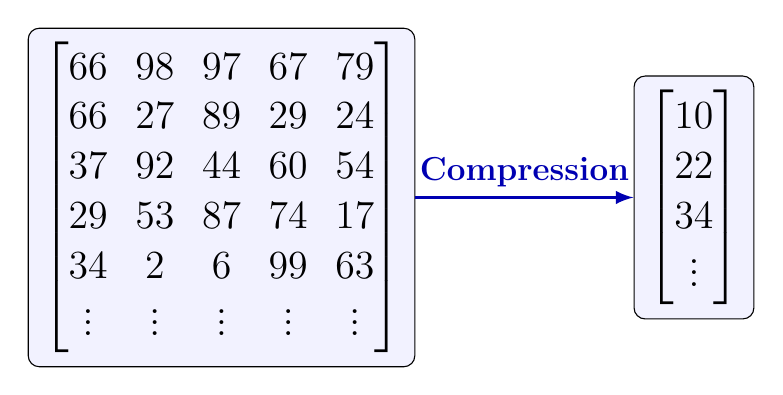
\begin{tikzpicture}[
            matrix/.style={font=\Large, draw, fill=blue!5!white, rounded corners, inner sep=5pt},
            arrow/.style={-latex, thick, color=blue!70!black, line width=1.2pt}
        ]
            % Input data matrix
            \node[matrix] (input) at (-3, 0) {\Large$\begin{bmatrix}
                66 & 98 & 97 & 67 & 79 \\
                66 & 27 & 89 & 29 & 24 \\
                37 & 92 & 44 & 60 & 54 \\
                29 & 53 & 87 & 74 & 17 \\
                34 & 2 & 6 & 99 & 63 \\
                \vdots & \vdots & \vdots & \vdots & \vdots
            \end{bmatrix}$};
            
            % Output features matrix
            \node[matrix] (output) at (3, 0) {\Large$\begin{bmatrix}
                10 \\
                22 \\
                34 \\
                \vdots
            \end{bmatrix}$};
            
            % Arrow
            \draw[arrow] (input.east) -- (output.west) node[midway, above, sloped, color=blue!70!black, font=\large] {\textbf{Compression}};
        \end{tikzpicture}
    \end{center}

    \vspace{0.5cm}
    \begin{tcolorbox}[colback=red!5!white, colframe=red!75!black, title=Why Use Compression?]
        \begin{itemize}
            \item \textbf{\textcolor{blue!70!black}{Efficiency:}} Reduces storage and computation requirements.
            \item \textbf{\textcolor{blue!70!black}{Focus:}} Highlights the most important patterns in data.
        \end{itemize}
    \end{tcolorbox}
\end{frame}


\begin{frame}{Introduction}
    \begin{tcolorbox}[colback=red!5!white, colframe=red!75!black, title=Objective]
        To minimize the reconstruction error between the input data (\(x\)) and the reconstructed output (\(\hat{x}\)).
    \end{tcolorbox}

    \vspace{0.3cm}

    \begin{tcolorbox}[colback=yellow!5!white, colframe=yellow!75!black, title=Applications]
        \begin{itemize}
            \item Dimensionality reduction
            \item Image denoising
            \item Anomaly detection
        \end{itemize}
    \end{tcolorbox}
    
\end{frame}


% Slide: Autoencoder Representation
\begin{frame}[t]{Autoencoder Architecture}
    \begin{center}
        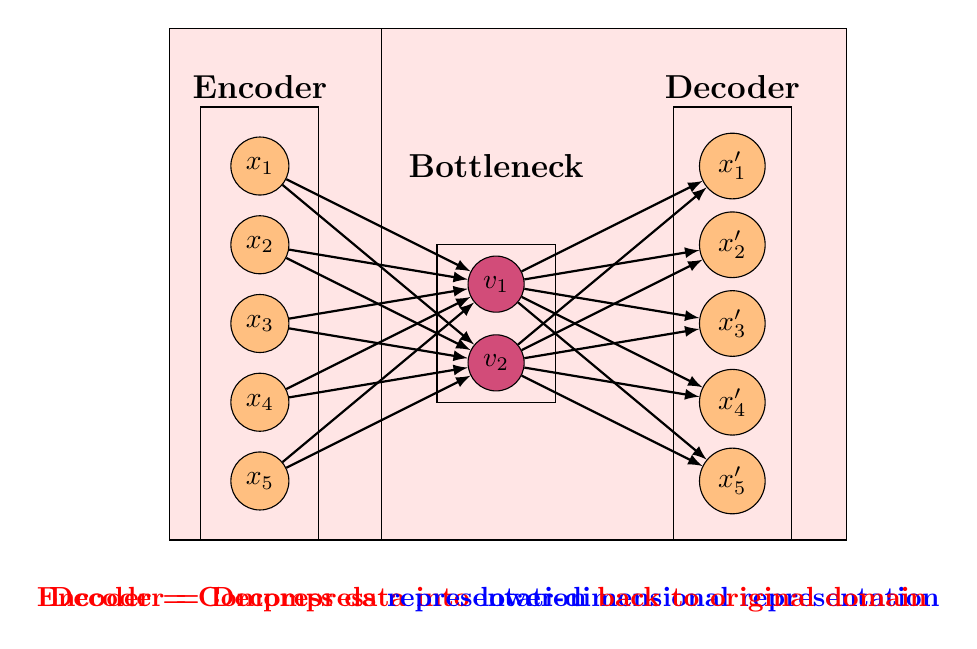
\begin{tikzpicture}[
            inputnode/.style={draw, circle, fill=orange!50, minimum size=12pt},
            hiddennode/.style={draw, circle, fill=purple!70, minimum size=12pt},
            outputnode/.style={draw, circle, fill=orange!50, minimum size=12pt},
            connection/.style={-latex, thick}
        ]

            % Encoder and Decoder Box
            \node<5>[draw, rectangle, minimum width=5.9cm, minimum height=6.5cm, fill=red!10] 
            (encoderbox) at (1.8, 0.5) {};
            \node<6>[draw, rectangle, minimum width=5.9cm, minimum height=6.5cm, fill=red!10] 
            (decoderbox) at (4.5, 0.5) {};

            % Titles
            \node<1,4->[align=center, font=\large\bfseries] at (0, 3) {Encoder};
            \node<2,4->[align=center, font=\large\bfseries] at (3, 2) {Bottleneck};
            \node<3,4->[align=center, font=\large\bfseries] at (6, 3) {Decoder};

            % Layer Boxes
            \node<1>[draw, rectangle, minimum width=1.5cm, minimum height=5.5cm, fill=red!10] 
            (inputbox) at (0, 0) {};
            \node<2>[draw, rectangle, minimum width=1.5cm, minimum height=2.0cm, fill=red!10] 
            (bottleneckbox) at (3, 0) {};
            \node<3>[draw, rectangle, minimum width=1.5cm, minimum height=5.5cm, fill=red!10] 
            (outputbox) at (6, 0) {};

            % Encoder and Decoder Descriptions
            \node<5>[align=center, text=red, font=\bfseries] at (2.9, -3.5) 
            {Encoder = Compress data into \textcolor{blue}{lower-dimensional representation}};
            \node<6>[align=center, text=red, font=\bfseries] at (2.9, -3.5) 
            {Decoder = Decompress \textcolor{blue}{representation} back to original domain};

            % Input Layer Nodes
            \node[inputnode] (x1) at (0, 2) {$x_1$};
            \node[inputnode] (x2) at (0, 1) {$x_2$};
            \node[inputnode] (x3) at (0, 0) {$x_3$};
            \node[inputnode] (x4) at (0, -1) {$x_4$};
            \node[inputnode] (x5) at (0, -2) {$x_5$};
            
            % Bottleneck Layer Nodes
            \node[hiddennode] (v1) at (3, 0.5) {$v_1$};
            \node[hiddennode] (v2) at (3, -0.5) {$v_2$};
            
            % Output Layer Nodes
            \node[outputnode] (y1) at (6, 2) {$x'_1$};
            \node[outputnode] (y2) at (6, 1) {$x'_2$};
            \node[outputnode] (y3) at (6, 0) {$x'_3$};
            \node[outputnode] (y4) at (6, -1) {$x'_4$};
            \node[outputnode] (y5) at (6, -2) {$x'_5$};
            
            % Connections: Input to Bottleneck
            \foreach \i in {1,2,3,4,5} {
                \draw[connection] (x\i) -- (v1);
                \draw[connection] (x\i) -- (v2);
            }
            
            % Connections: Bottleneck to Output
            \foreach \j in {1,2,3,4,5} {
                \draw[connection] (v1) -- (y\j);
                \draw[connection] (v2) -- (y\j);
            }
           
        \end{tikzpicture}
    \end{center}
\end{frame}

\begin{frame}{Impact of Latent Dimension}
    \begin{itemize}
        \item \textcolor{orange!80!black}{As the number of neurons increases}, the number of latent dimensions also increases.
        \item \textcolor{blue!80!black}{Similar class instances} are mapped to similar regions in the latent space.
        \item \textcolor{red}{In lower dimensions}, latent space is \textbf{not that much organized} with overlapping clusters.
        \item \textcolor{green!60!black}{In Higher dimensions}, the clusters are much more separated.
    \end{itemize}
    \vspace{0.3cm}
    \begin{tcolorbox}[colback=blue!5!white, colframe=blue!75!black, sharp corners=all, boxrule=0.8mm]
        \textbf{Conclusion:}
        \begin{itemize}
            \item Higher-dimensional latent spaces enable \textbf{better cluster separation}.
            \item Reconstruction accuracy improves as the latent dimension increases.
        \end{itemize}
    \end{tcolorbox}
\end{frame}




% Slide 2: Importance of Latent Dimension
\begin{frame}{Latent Space Comparison}
    \begin{center}
        % Two images side by side
        \begin{minipage}{0.45\linewidth}
            \centering
            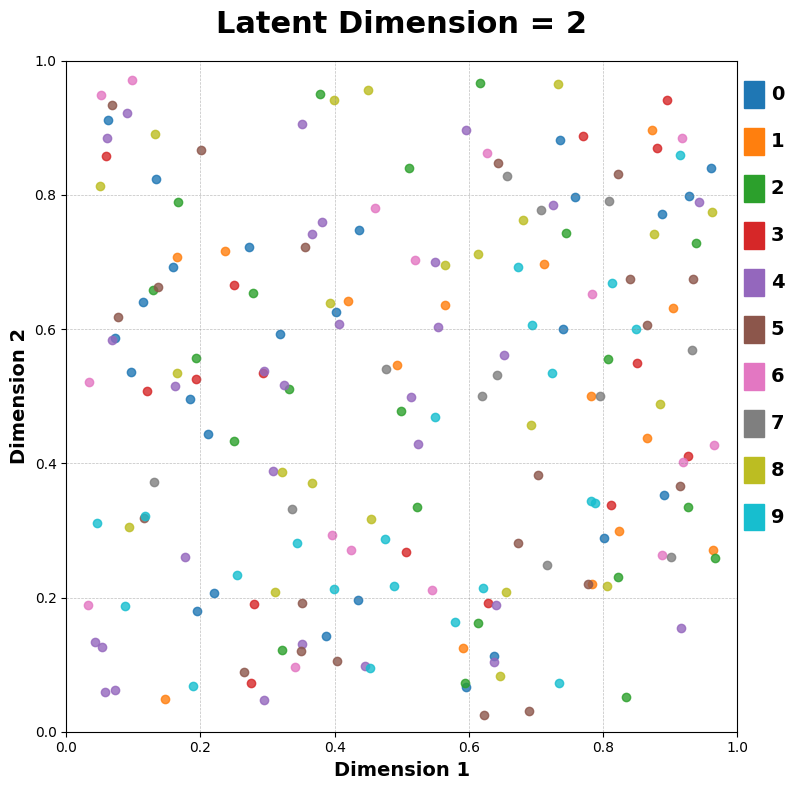
\includegraphics[width=\linewidth]{light_theme_animation/frame_001.png} % Path to the 2D latent space image
            \vspace{0.2cm}
            \textbf{\textcolor{red}{Lower Dimension}}
        \end{minipage}
        \hfill
        \begin{minipage}{0.45\linewidth}
            \centering
            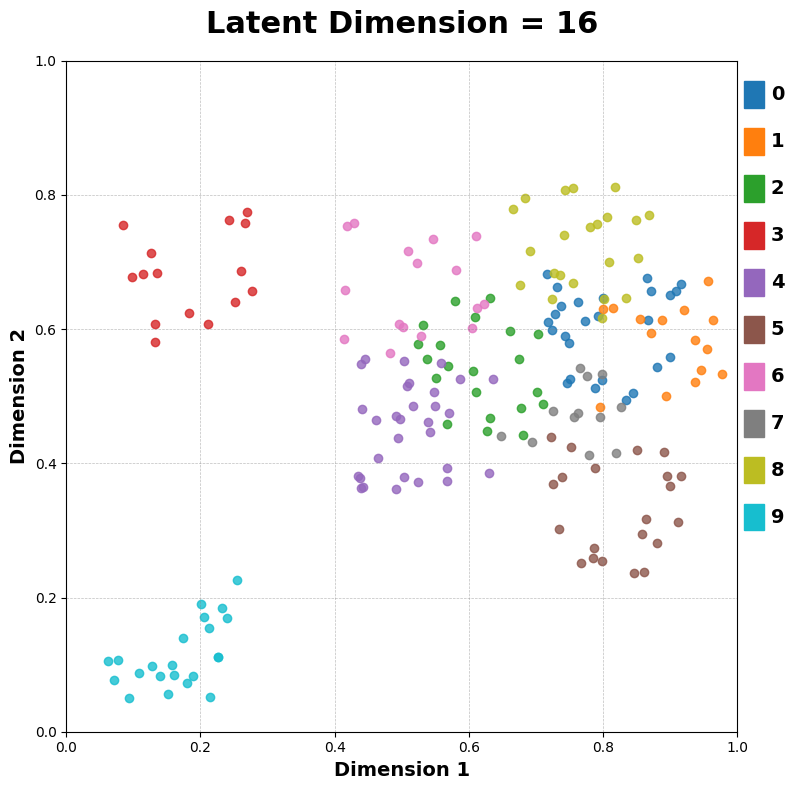
\includegraphics[width=\linewidth]{light_theme_animation/frame_015.png} % Path to the 5D latent space image
            \vspace{0.2cm}
            \textbf{\textcolor{green!60!black}{Higher Dimension }}
        \end{minipage}
    \end{center}
    \vspace{0.3cm}
    \begin{itemize}
        \item \textcolor{red}{In lower dimensions}, clusters for digits like \textbf{1} and \textbf{5} \textbf{overlap}.
        \item \textcolor{green!60!black}{In higher dimensions}, clusters are \textbf{distinct} like \textbf{8} is in the top-right corner, and \textbf{9} is separated below.
       
    \end{itemize}
    \vspace{0.3cm}
    \begin{tcolorbox}[colback=yellow!10!white, colframe=orange!80!black, sharp corners=all, boxrule=0.8mm]
        \textbf{Key Insight:} Higher dimensions allow better separation of clusters and more accurate data reconstruction.
    \end{tcolorbox}
\end{frame}






\begin{frame}[t]{Plot with Latent Dimension}
    \begin{center}
        % Corrected animategraphics command
        \animategraphics[autoplay,loop,width=0.60\linewidth]{4}{light_theme_animation/frame_}{001}{018}
    \end{center}
    \vspace{-2cm}
    \begin{center}
        \textit{Training reduces loss over time.}
    \end{center}
\end{frame}

\begin{frame}{Comparison of Initial and Final Stages}
    \begin{center}
        % Two images side by side
        \begin{minipage}{0.45\linewidth}
            \centering
            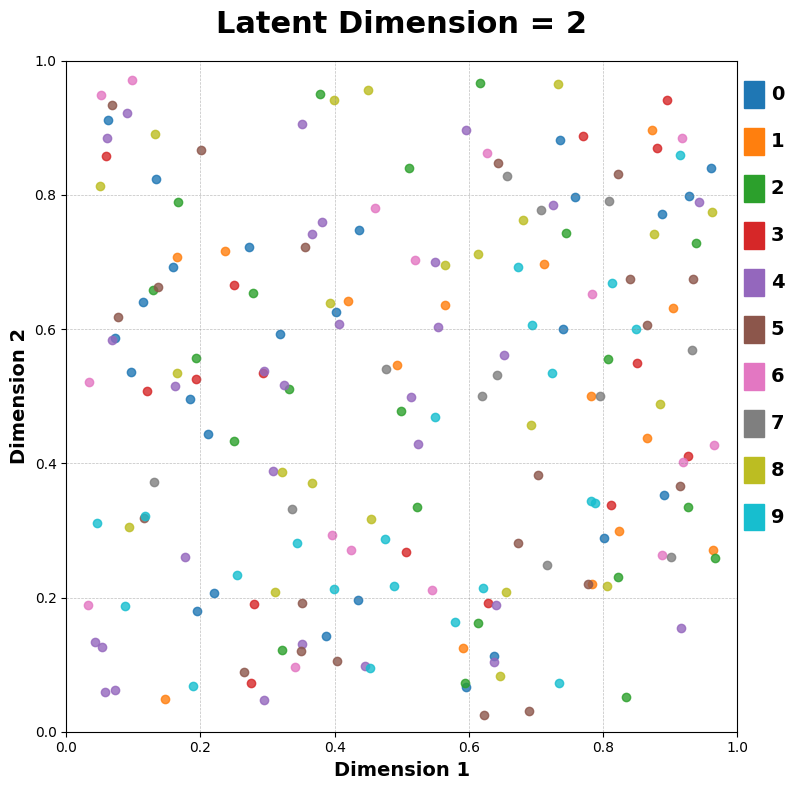
\includegraphics[width=\linewidth]{light_theme_animation/frame_001} % Path to the initial stage image
            \vspace{0.2cm}
            \textbf{Initial Stage}
        \end{minipage}
        \hfill
        \begin{minipage}{0.45\linewidth}
            \centering
            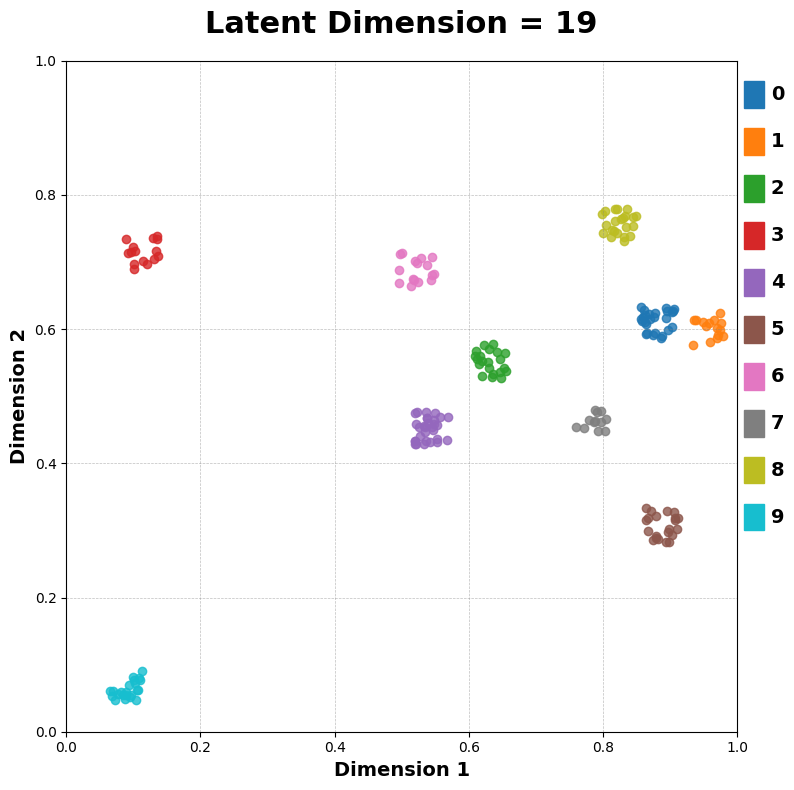
\includegraphics[width=\linewidth]{light_theme_animation/frame_018} % Path to the final stage image
            \vspace{0.2cm}
            \textbf{Final Stage}
        \end{minipage}
    \end{center}
    \vspace{0.5cm}
    \begin{center}
        Observe the transformation from the initial stage to the final stage of training.
    \end{center}
\end{frame}


\begin{frame}{How Autoencoders Process Data}
\scalebox{0.7}{
    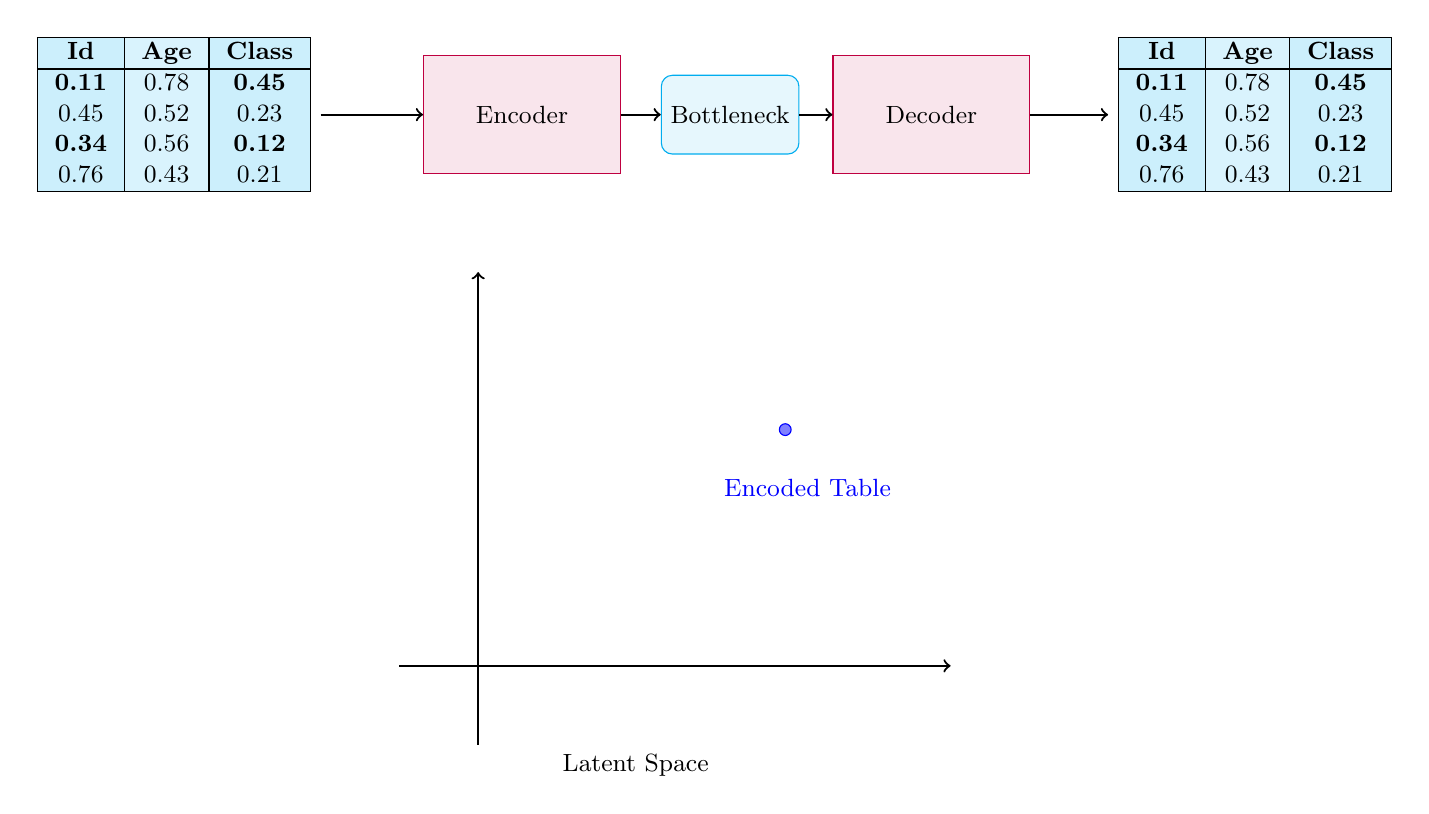
\begin{tikzpicture}[every node/.style={font=\small}, node distance=1.5cm, auto]

        % Input matrix (4x3 table with headers)
        \node[anchor=east] (input) at (0, -2) 
        {
        \begin{tabular}{|>{\columncolor{cyan!20}}c|>{\columncolor{cyan!15}}c|>{\columncolor{cyan!20}}c|}
            \hline
            \textbf{Id} & \textbf{Age} & \textbf{Class} \\
            \hline
            \textbf{0.11} & 0.78 & \textbf{0.45} \\
            0.45 & 0.52 & 0.23 \\
            \textbf{0.34} & 0.56 & \textbf{0.12} \\
            0.76 & 0.43 & 0.21 \\
            \hline
        \end{tabular}
        };

        % Encoder (rectangle)
        \node[draw=purple, fill=purple!10, minimum height=1.5cm, 
        minimum width=2.5cm, anchor=west] (encoder) at (1.3, -2) {Encoder};

        % Bottleneck (latent space)
        \node[rectangle, draw=cyan, fill=cyan!10, minimum width=1.5cm, 
        minimum height=1cm, rounded corners] (bottleneck) at (5.2, -2) {Bottleneck};

        % Decoder (rectangle)
        \node[draw=purple, fill=purple!10, minimum height=1.5cm, 
        minimum width=2.5cm, anchor=west] (decoder) at (6.5, -2) {Decoder}; 

        % Output matrix (4x3 table with headers)
        \node[anchor=west] (output) at (10, -2) 
        {
        \begin{tabular}{|>{\columncolor{cyan!20}}c|>{\columncolor{cyan!15}}c|>{\columncolor{cyan!20}}c|}
            \hline
            \textbf{Id} & \textbf{Age} & \textbf{Class} \\
            \hline
            \textbf{0.11} & 0.78 & \textbf{0.45} \\
            0.45 & 0.52 & 0.23 \\
            \textbf{0.34} & 0.56 & \textbf{0.12} \\
            0.76 & 0.43 & 0.21 \\
            \hline
        \end{tabular}
        };

        % Arrows connecting components
        \draw[->, thick] (input.east) -- (encoder.west);
        \draw[->, thick] (encoder.east) -- (bottleneck.west);
        \draw[->, thick] (bottleneck.east) -- (decoder.west);
        \draw[->, thick] (decoder.east) -- (output.west);

        % Latent space axes
        \draw[->, thick] (2, -10) -- (2, -4);
        \node[below] at (4, -10) {Latent Space};
        \draw[->, thick] (1, -9) -- (8, -9);

       {\textcolor{red}{Encoded data}};
        % Encoded table point
        \node[circle, draw=blue, fill=blue!50, inner sep=1.5pt] at (5.9, -6) {};
        \node[below right] at (5, -6.5) {\textcolor{blue}{Encoded Table}};
    \end{tikzpicture}
    }
\end{frame}



\begin{frame}{How Autoencoders Process Data}
\scalebox{0.7}{
    \begin{tikzpicture}[every node/.style={font=\small}, node distance=1.5cm, auto]

        % Input image
        \node[anchor=east] (input) at (0, -2) 
        {
            \includegraphics[width=3cm]{dataprocess.jpg}  % Change the file path and name
        };

        % Encoder (rectangle)
        \node[draw=purple, fill=purple!10, minimum height=1.5cm, 
        minimum width=2.5cm, anchor=west] (encoder) at (1.3, -2) {Encoder};

        % Bottleneck (latent space)
        \node[rectangle, draw=cyan, fill=cyan!10, minimum width=1.5cm, 
        minimum height=1cm, rounded corners] (bottleneck) at (5.2, -2) {Bottleneck};

        % Decoder (rectangle)
        \node[draw=purple, fill=purple!10, minimum height=1.5cm, 
        minimum width=2.5cm, anchor=west] (decoder) at (6.5, -2) {Decoder}; 

        % Output image
        \node[anchor=west] (output) at (10, -2) 
        {
            \includegraphics[width=3cm]{dataprocess.jpg}  % Change the file path and name
        };

        % Arrows connecting components
        \draw[->, thick] (input.east) -- (encoder.west);
        \draw[->, thick] (encoder.east) -- (bottleneck.west);
        \draw[->, thick] (bottleneck.east) -- (decoder.west);
        \draw[->, thick] (decoder.east) -- (output.west);

        % Latent space axes
        \draw[->, thick] (2, -10) -- (2, -4);
        \node[below] at (4, -10) {Latent Space};
        \draw[->, thick] (1, -9) -- (8, -9);

        % Encoded data point
        \node[circle, draw=red, fill=red!50, inner sep=1.5pt] at (3.3, -5) {};
        \node[below right] at (3, -5.5) {\textcolor{red}{Encoded Image}};
        
        
    \end{tikzpicture}
}
\end{frame}


\begin{frame}{Before and After Reconstruction}
    \begin{columns}[T,onlytextwidth]
        \begin{column}{0.48\textwidth}
            \centering
            \includegraphics[width=0.8\linewidth]{before_after.png} % Replace with the original image path
            \vspace{0.3cm}
            \newline
            \textbf{\color{blue}Original Image}
        \end{column}
        \begin{column}{0.48\textwidth}
            \centering
            \includegraphics[width=0.8\linewidth]{before_after.png} % Replace with the reconstructed image path
            \vspace{0.3cm}
            \newline
            \textbf{\color{blue}Reconstructed Image}
        \end{column}
    \end{columns}

    \vspace{0.5cm}
    \begin{tcolorbox}[
        colback=blue!9!white, 
        colframe=blue!75!black, 
        sharp corners,
        title= Main Goal,
        fonttitle=\bfseries\large,
        width=\textwidth,
        boxrule=0.5mm
    ]
        Minimize the difference between the original and reconstructed images.
    \end{tcolorbox}
   .
\end{frame}


\begin{frame}{Loss Function and Key Metrics}
    \vspace{-.1cm}
    \begin{tcolorbox}[
        colback=yellow!10!white, 
        colframe=orange!85!black, 
        sharp corners,
        title=\textbf{Mathematical Equation},
        fonttitle=\bfseries\large,
        width=\textwidth,
        boxrule=0.5mm
    ]
        \[
        \mathcal{L} = \frac{1}{N} \sum_{i=1}^{N} \| x_i - \hat{x}_i \|^2
        \]
    \end{tcolorbox}
    
    \vspace{0.4cm}
    \textbf{Where:}
    \begin{itemize}
        \item \textbf{\( x \)}: \textcolor{blue}{Original input image}
        \item \textbf{\( \hat{x} \)}: \textcolor{blue}{Reconstructed image}
        \item \textbf{\( \| \cdot \|^2 \)}: \textcolor{red}{Squared Euclidean distance (error)}
    \end{itemize}

    \vspace{0.3cm}
    \begin{tcolorbox}[
        colback=green!5!white, 
        colframe=green!75!black, 
        sharp corners,
        title=\textbf{Key Insight},
        fonttitle=\bfseries\large,
        width=\textwidth,
        boxrule=0.5mm
    ]
        \textbf{\color{purple}Optimization:} Reduce loss to improve reconstruction quality.\newline
        \textbf{\color{purple}Takeaway:} Small loss = Better reconstruction!
    \end{tcolorbox}
    
    \vspace{0.3cm}
    \textbf{\color{blue}Takeaway:} Small loss = Better reconstruction!
\end{frame}

\begin{frame}{Key Focus of Autoencoder Training}
    \begin{tcolorbox}[colback=purple!5!white, colframe=purple!75!black, width=\textwidth, sharp corners=all, boxrule=1mm]
        \textbf{Decoder's Goal:} Improve its ability to accurately reconstruct the original data from the compressed representation.
    \end{tcolorbox}
    \vspace{0.5cm}
    \begin{tcolorbox}[colback=orange!5!white, colframe=orange!75!black, width=\textwidth, sharp corners=all, boxrule=1mm]
        \textbf{Encoder's Goal:} Learn to compress data in a way that preserves critical information for reconstruction.
    \end{tcolorbox}
\end{frame}




% Animated Slide: Training Loss
\begin{frame}[t]{Training Loss Animation}
    \begin{center}
        \animategraphics[autoplay,loop,width=0.8\linewidth]{4}{animation_image/loss_frame_}{1}{20}
    \end{center}
    \vspace{0.5cm}
    \begin{center}
        \textit{Training reduces loss over time, as shown above.}
    \end{center}
\end{frame}




\usetikzlibrary{shapes.geometric, arrows}

% Define TikZ styles
\tikzstyle{startstop} = [ellipse, minimum width=3cm, minimum height=1.7cm, text centered, draw=red!70, fill=red!30]
\tikzstyle{process} = [rectangle, minimum width=3.5cm, minimum height=1cm, text centered, draw=blue!70, fill=blue!30, rounded corners]
\tikzstyle{box} = [rectangle, minimum width=6cm, minimum height=7cm, text centered, draw=red!70, fill=yellow!10, rounded corners]
\tikzstyle{decision} = [diamond, minimum width=3.5cm, minimum height=1cm, text centered, draw=orange!70, fill=yellow!40]
\tikzstyle{data} = [trapezium, trapezium left angle=70, trapezium right angle=110, minimum width=3.5cm, minimum height=1cm, text centered, draw=green!90, fill=green!40]
\tikzstyle{arrow} = [thick,->,>=stealth]

% Flowchart slide
\begin{frame}{Autoencoder Training Process}
    \begin{center}
        \scalebox{0.7}{ % Scale down the entire diagram 
        \begin{tikzpicture}[node distance=2.5cm and 3.5cm]

            % Nodes
            \node (start) [startstop] {Start};\pause
             \draw [arrow] (start) -- (input);
            \node (input) [data, right of=start, xshift = 3 cm] {Generate Input Data};\pause
             \draw [arrow] (input) -- (encoder);
            \node (box) [box, below of = input, yshift = -2.5cm]{};
            \node (encoder) [process, below of=input,  fill=yellow!40, draw=orange!90] {Pass through Encoder};
            \node (bottleneck) [process, below of=encoder,  fill=yellow!40, draw=orange!90] {Compressed Representation};
            \node (decoder) [process, below of=bottleneck,  fill=yellow!40, draw=orange!90] {Pass through Decoder};
            \draw [arrow] (encoder) -- (bottleneck);
            \draw [arrow] (bottleneck) -- (decoder);
            \draw [arrow] (decoder) -- (output);\pause
            \node (output) [process, below of=decoder] {Reconstructed Output Data};\pause
            \node (compare) [process, left of=output, xshift=-4.5cm, ] {Compare Output with Input};
             \draw [arrow] (output) -- (compare);\pause
            \node (decision) [decision, above of=compare, yshift=1.5cm] {Is Loss Acceptable?};
             \draw [arrow] (decision) -- node[anchor=south] {Yes} (end);
            \node (end) [startstop, left of=decision, xshift=-2cm] {End};
            
            \draw [arrow] (decision.north) |- (adjust.south) node[midway, right, yshift=-0.4cm] {No};
            \node (adjust) [process, above of=decision, yshift=1cm, fill=blue!30, draw=blue!90] {Adjust Model};
           

            

            % Arrows
            \draw [arrow] (compare) -- (decision);
            \draw [arrow] (decision) -- node[anchor=south] {Yes} (end);
            \draw [arrow] (decision.north) |- (adjust.south) node[midway, right, yshift=-0.4cm] {No};
            \draw [arrow] (adjust) -- (encoder);

        \end{tikzpicture}
        }
    \end{center}
\end{frame}



% ABHISHEK ROY - 2105033


\begin{frame}{Basic Autoencoder}
    \begin{tcolorbox}[colback=blue!5!white, colframe=blue!75!black, fonttitle=\small, fontupper=\footnotesize, title=Overview]
        An \textbf{Autoencoder} is a type of model that takes an input vector \( \mathbf{x} \), compresses it into a lower-dimensional \textbf{Latent Space} representation \( \mathbf{z} \), and then reconstructs the input vector \( \mathbf{x} \) from \( \mathbf{z} \).
    \end{tcolorbox}

    \begin{center}
        \begin{figure}
            \centering
            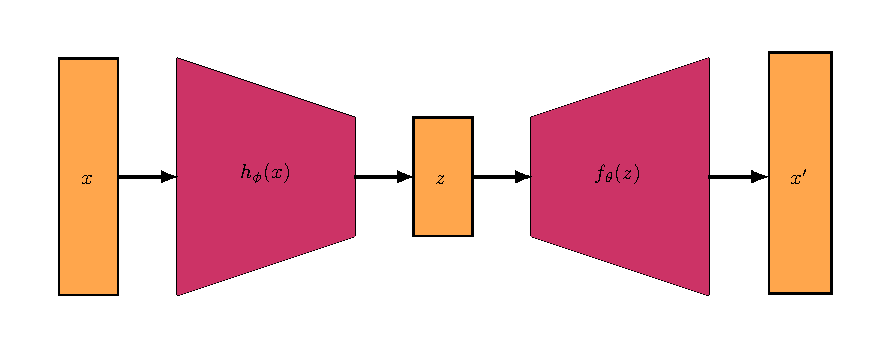
\includegraphics[width=10cm]{./TIKZ_TEX_FILE/PDFS/basic_auto.pdf}
            \caption{Architecture of an AutoEncoder}
            \label{fig:enter-label}
        \end{figure}
    \end{center}
\end{frame}

\begin{frame}{Purpose of Autoencoder}
    \begin{center}
        \begin{figure}
            \centering
            \includegraphics[width=12cm]{img/pic1.png}
            \label{fig:enter-label}
        \end{figure}
    \end{center}
\end{frame}

\begin{frame}{Limitations of Traditional Autoencoders}
    \begin{tcolorbox}[colback=red!5!white, colframe=red!80!black, title=Disadvantages, fonttitle=\small, fontupper=\footnotesize]
        \begin{itemize}
            \item \textbf{\textcolor{red}{Overfitting Risk:}} May not generalize well on unseen data.
            \item \textbf{\textcolor{red}{Lack of Probabilistic Structure:}} Do not model uncertainty in the data.
            \item \textbf{\textcolor{red}{Lack of Structure in Latent Space:}} Latent space may not be well-structured or interpretable.
        \end{itemize}
    \end{tcolorbox}

    \vspace{1em}
    
    \begin{tcolorbox}[colback=teal!5!white, colframe=teal!80!black, title=Solution, fonttitle=\small, fontupper=\footnotesize]
    \textbf{\textcolor{teal}{Variational Autoencoders (VAEs)}} address these issues by introducing a 
    \textbf{\textcolor{teal}{Probabilistic Framework}} and ensuring a 
    \textbf{\textcolor{teal}{Structured Latent Space}} for 
    \textbf{\textcolor{teal}{Better Generalization}}.
\end{tcolorbox}
\end{frame}

\begin{frame}{Variational AutoEncoder}
    \begin{tcolorbox}[colback=blue!5!white, colframe=blue!75!black, fonttitle=\small, fontupper=\footnotesize]
        \textbf{Variational AutoEncoders (VAEs)} were proposed in the paper \textbf{\textit{"Auto-Encoding Variational Bayes"}} by \textbf{Diederik P. Kingma} and \textbf{Max Welling} (2013).
    \end{tcolorbox}

    \vspace{1em}
    \begin{columns}[c]
        \column{0.4\textwidth}
        \begin{center}
            \includegraphics[width=0.5\textwidth]{img/VaePaper.png} \\[0.5em]
            \footnotesize \textit{Auto-Encoding Variational Bayes}
        \end{center}

        \column{0.4\textwidth}
        \begin{center}
            \includegraphics[width=0.5\textwidth]{img/kingma.jpg} \\[0.5em]
            \footnotesize \textit{Diederik P. Kingma}
        \end{center}
    \end{columns}
\end{frame}



\begin{frame}{Neural Network Representation of Auto Encoder}
    \begin{figure}
        \centering
        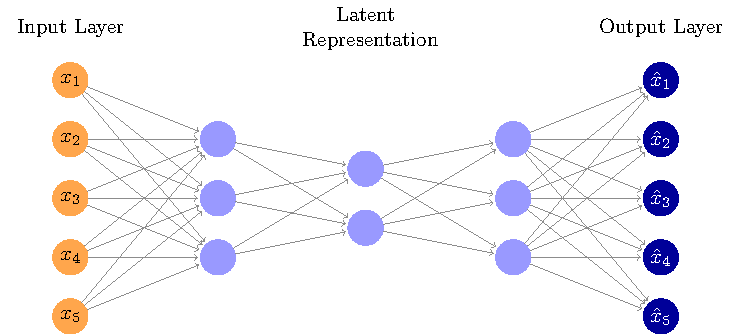
\includegraphics[width=\linewidth]{./TIKZ_TEX_FILE/PDFS/auto_nn.pdf}
        \caption{A Standard Autoencoder}
        \label{fig:enter-label}
    \end{figure}
\end{frame}


\begin{frame}{Neural Network Representation of VAE}
    \begin{figure}
        \centering
        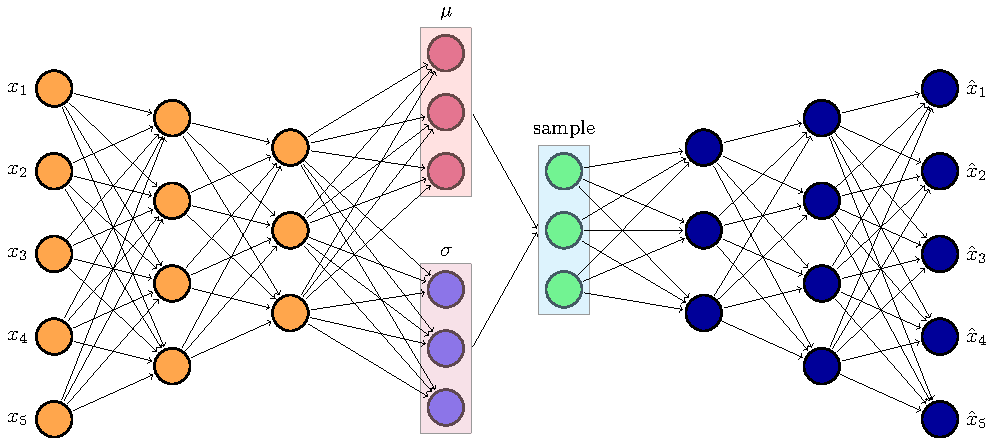
\includegraphics[width=\linewidth]{./TIKZ_TEX_FILE/PDFS/vae_nn.pdf}
        \caption{A Standard Variational Autoencoder}
        \label{fig:enter-label}
    \end{figure}
\end{frame}


\begin{frame}{High Level Block Diagram of VAE}
    \begin{figure}
        \centering
        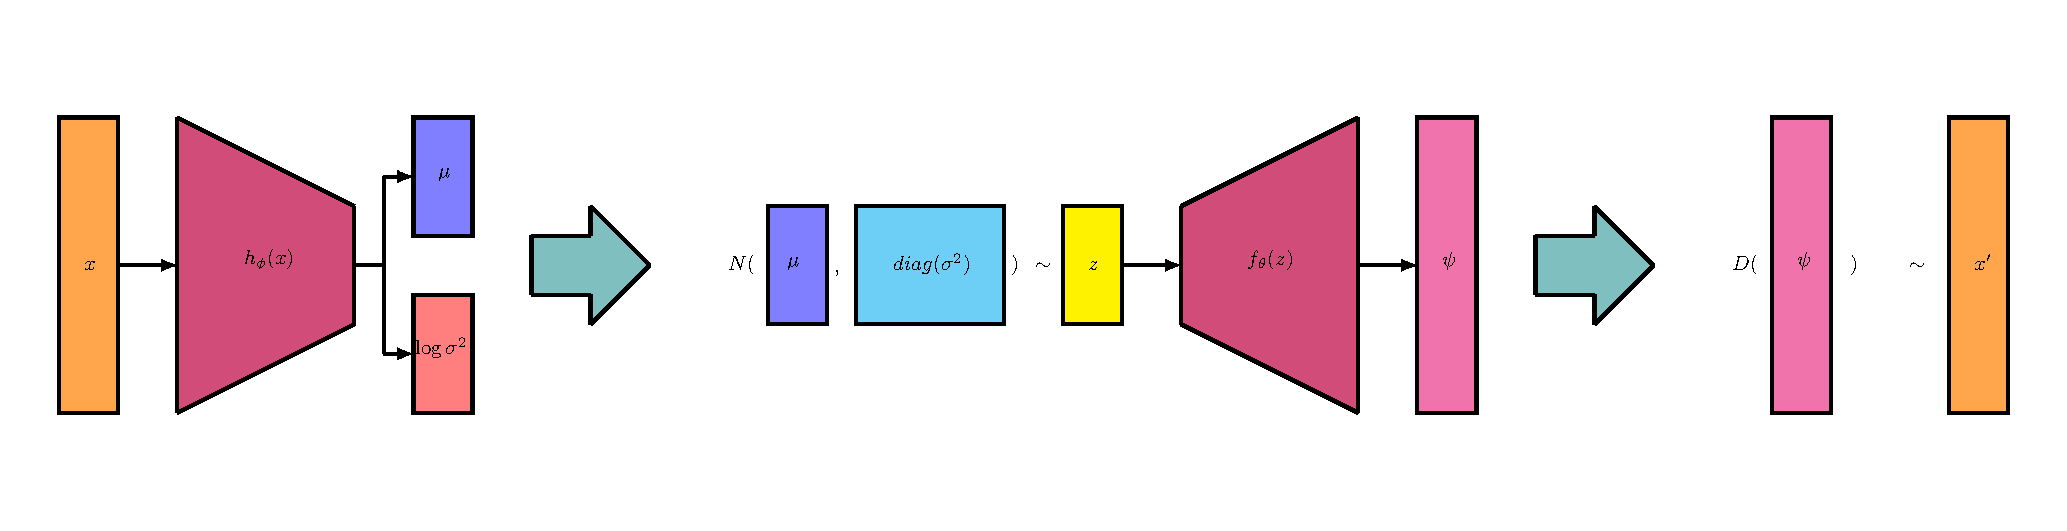
\includegraphics[width=12cm]{./TIKZ_TEX_FILE/PDFS/high_vae.pdf}
        \caption{High Level Architechture of an VAE}
        \label{fig:enter-label}
    \end{figure}
\end{frame}

\begin{frame}
    \begin{center}
        \Large
        Hard to understand? yeah same
    \end{center}    
\end{frame}

\begin{frame}{VAE Simplified}
    \begin{figure}
        \centering
        \includegraphics[width=12cm]{img/2.png}
        \caption{Probabilistic Distribution Encoding}
        \label{fig:enter-label}
    \end{figure}
\end{frame}

\begin{frame}{VAE Simplified}
    \begin{figure}
        \centering
        \includegraphics[width=12cm]{img/pic3.png}
        \caption{Generating Clean Picture}
        \label{fig:enter-label}
    \end{figure}
\end{frame}

\begin{frame}{VAE Simplified}
    \begin{figure}
        \centering
        \includegraphics[width=12cm]{img/pic4.png}
        \caption{Accurate Generate/Reconstruction from Latent Attributes}
        \label{fig:enter-label}
    \end{figure}
\end{frame}

% Slide 1: Input x
\begin{frame}{Input}
    \begin{center}
        \begin{tikzpicture}
            \node[anchor=south west, inner sep=0] (image) at (0,0) {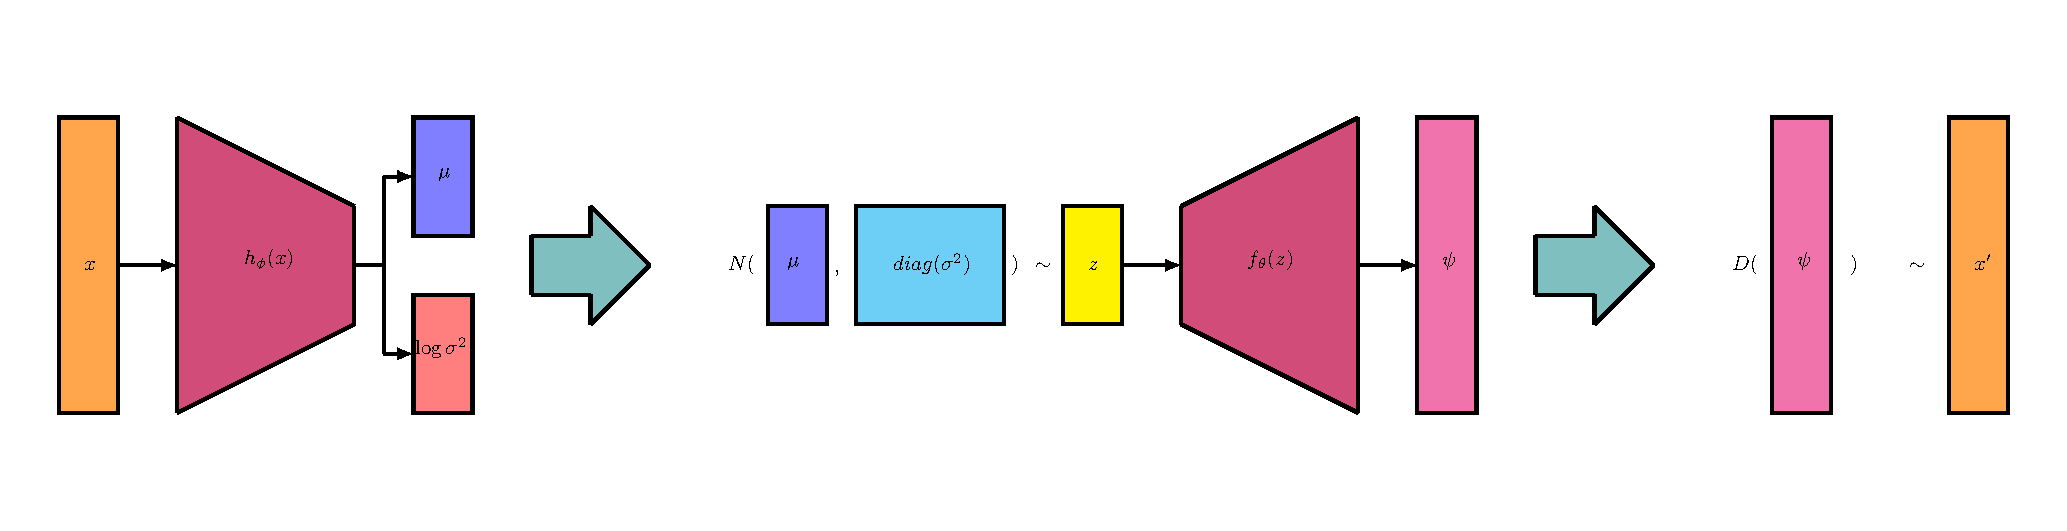
\includegraphics[width=12cm]{./TIKZ_TEX_FILE/PDFS/high_vae.pdf}};
        
            \begin{scope}[x={(image.south east)},y={(image.north west)}]
        
            
            \draw[red, thick] (0.02, 0.2) rectangle (0.065, 0.8);
            \draw[red, thick, fill, opacity=0.15] (0.02, 0.2) rectangle (0.065, 0.8);
        
            \end{scope}
        \end{tikzpicture} 
    \end{center}    

    \pause
    
    \begin{tcolorbox}[colback=blue!5!white, colframe=blue!75!black, fonttitle=\small, fontupper=\footnotesize]
        The \textbf{Variational Autoencoder} begins with an input sample \textbf{\( x \)}, which can be an \textbf{image}, \textbf{text}, or any \textbf{data}.
    \end{tcolorbox}     
\end{frame}

% Slide 2: Encoder
\begin{frame}{Encoder}
    \begin{center}
        \begin{tikzpicture}
            \node[anchor=south west, inner sep=0] (image) at (0,0) {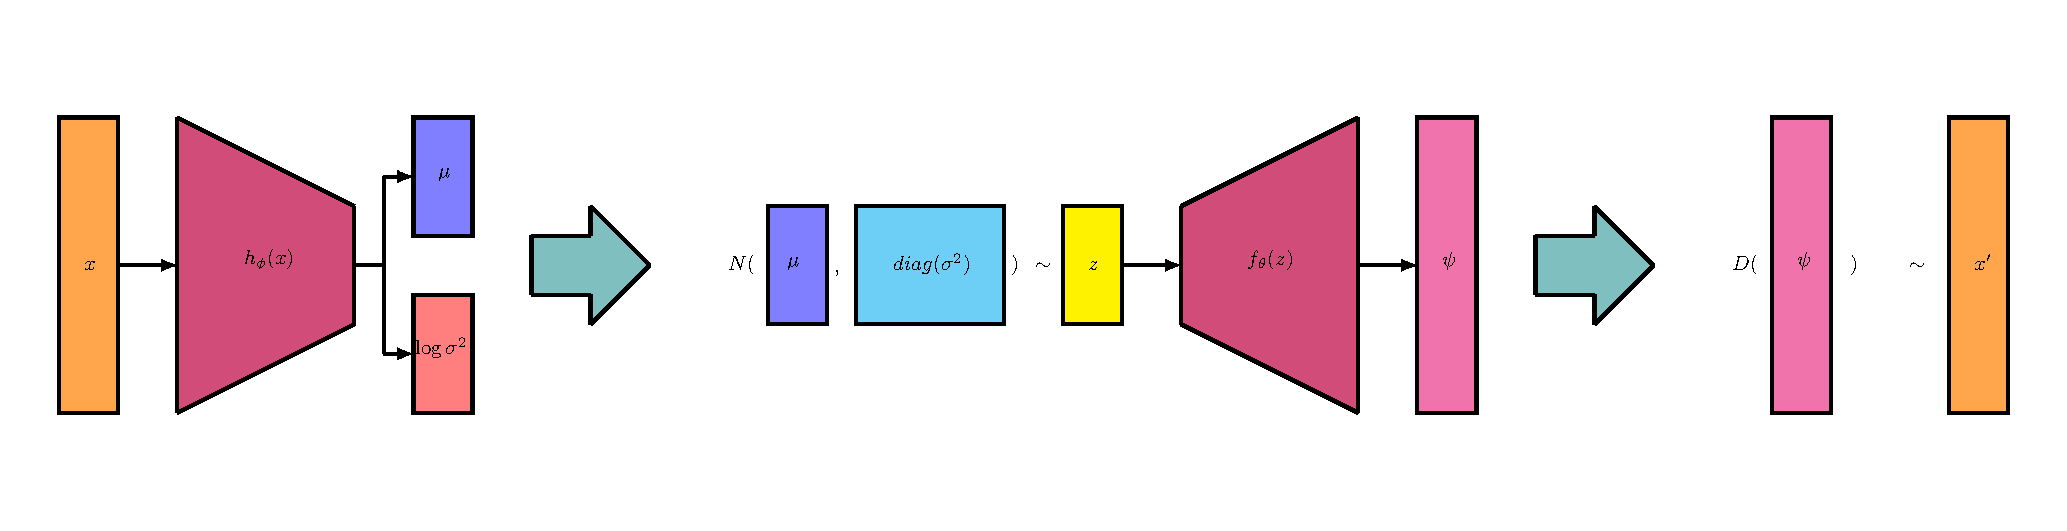
\includegraphics[width=12cm]{./TIKZ_TEX_FILE/PDFS/high_vae.pdf}};
        
            \begin{scope}[x={(image.south east)},y={(image.north west)}]
        
            
            \draw[red, thick] (0.08, 0.2) rectangle (0.25, 0.8);
            \draw[red, thick, fill, opacity=0.15] (0.08, 0.2) rectangle (0.25, 0.8);
            % \node[red, font=\small] at (0.3, 0.72) {Highlighted Area};
        
            \end{scope}
        \end{tikzpicture} 
    \end{center}

    \pause 
    
    \begin{tcolorbox}[colback=blue!5!white, colframe=blue!75!black, fonttitle=\small, fontupper=\footnotesize]
        \begin{itemize}
        \item The \textbf{Encoder} maps the input \( x \) into a \textbf{Latent Space Representation}.
        \item Outputs:
            \begin{itemize}
                \item \textbf{Mean (\( \mu \))}.
                \item \textbf{Log Variance (\( \log \sigma^2 \))}.
            \end{itemize}
    \end{itemize}
    \end{tcolorbox} 
    
\end{frame}

% Slide 3: Latent Variable z
\begin{frame}{Latent Variable}
    \begin{center}
        \begin{tikzpicture}
            \node[anchor=south west, inner sep=0] (image) at (0,0) {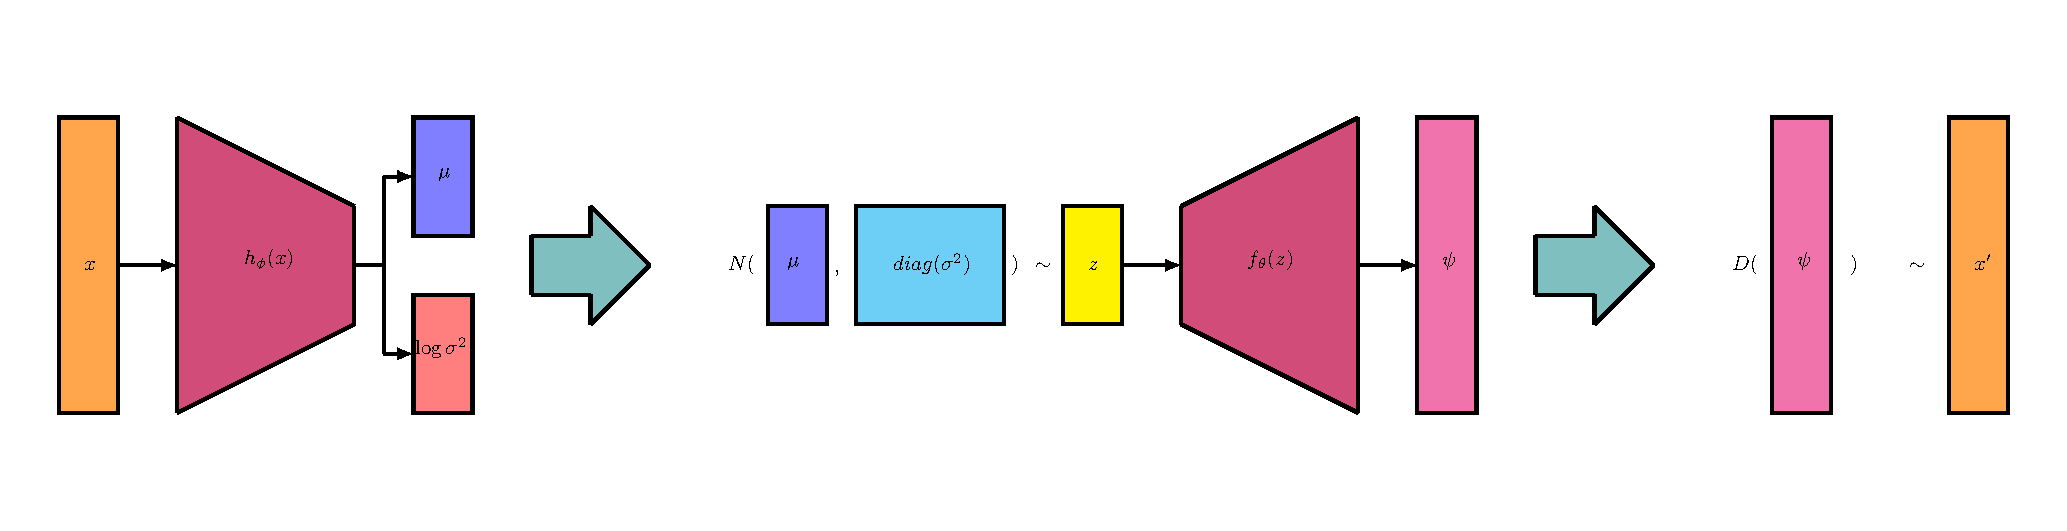
\includegraphics[width=12cm]{./TIKZ_TEX_FILE/PDFS/high_vae.pdf}};
        
            \begin{scope}[x={(image.south east)},y={(image.north west)}]
        
            
            \draw[red, thick] (0.35, 0.2) rectangle (0.55, 0.8);
            \draw[red, thick, fill, opacity=0.15] (0.35, 0.2) rectangle (0.55, 0.8);
            % \node[red, font=\small] at (0.3, 0.72) {Highlighted Area};
        
            \end{scope}
        \end{tikzpicture} 
    \end{center}
    
    \pause

    \begin{tcolorbox}[colback=blue!5!white, colframe=blue!75!black, fonttitle=\small, fontupper=\footnotesize]
        \( z \) represents a compressed \textbf{probabilistic latent space}.
    \end{tcolorbox}     

    \pause 
    
    \begin{tcolorbox}[colback=blue!5!white, colframe=blue!75!black, fonttitle=\small, fontupper=\footnotesize]
        Instead of fixed values, \( z \) is drawn from a distribution defined by the encoder: 
        \[
        p(z \mid x) \sim \mathcal{N}(\mu, \sigma^2).
        \]
    \end{tcolorbox}  
\end{frame}

% Slide 4: Decoder
\begin{frame}{Decoder}
    \begin{center}
        \begin{tikzpicture}
            \node[anchor=south west, inner sep=0] (image) at (0,0) {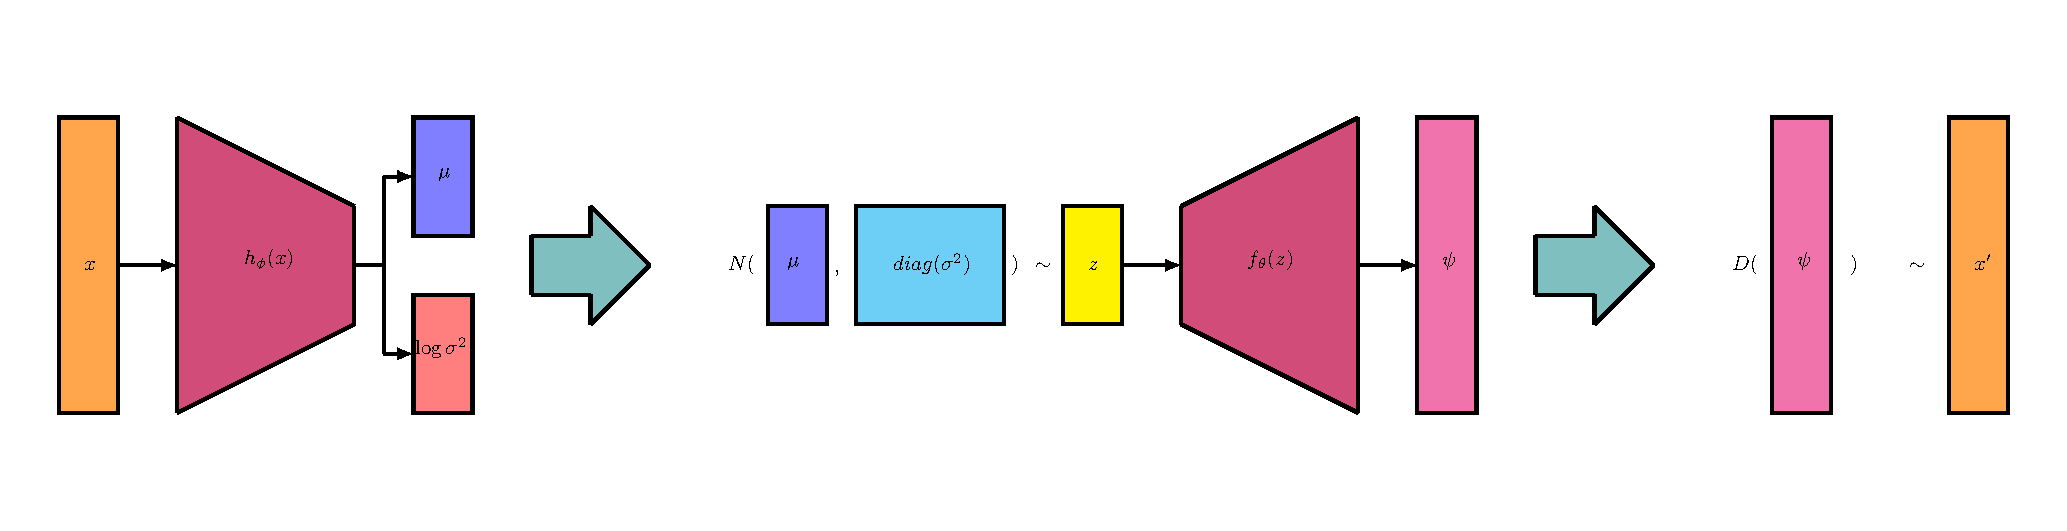
\includegraphics[width=12cm]{./TIKZ_TEX_FILE/PDFS/high_vae.pdf}};
        
            \begin{scope}[x={(image.south east)},y={(image.north west)}]
        
            
            \draw[red, thick] (0.56, 0.2) rectangle (0.73, 0.8);
            \draw[red, thick, fill, opacity=0.15] (0.56, 0.2) rectangle (0.73, 0.8);
            % \node[red, font=\small] at (0.3, 0.72) {Highlighted Area};
        
            \end{scope}
        \end{tikzpicture} 
    \end{center}

    \pause

    \begin{tcolorbox}[colback=blue!5!white, colframe=blue!75!black, fonttitle=\small, fontupper=\footnotesize]
        The decoder maps \( z \) to reconstructed data \( x' \) via \( p_\theta(x | z) \).  
    \end{tcolorbox}
    
    
\end{frame}

% Slide 5: Output
\begin{frame}{Output: \( x' \)}
    \begin{center}
        \begin{tikzpicture}
            \node[anchor=south west, inner sep=0] (image) at (0,0) {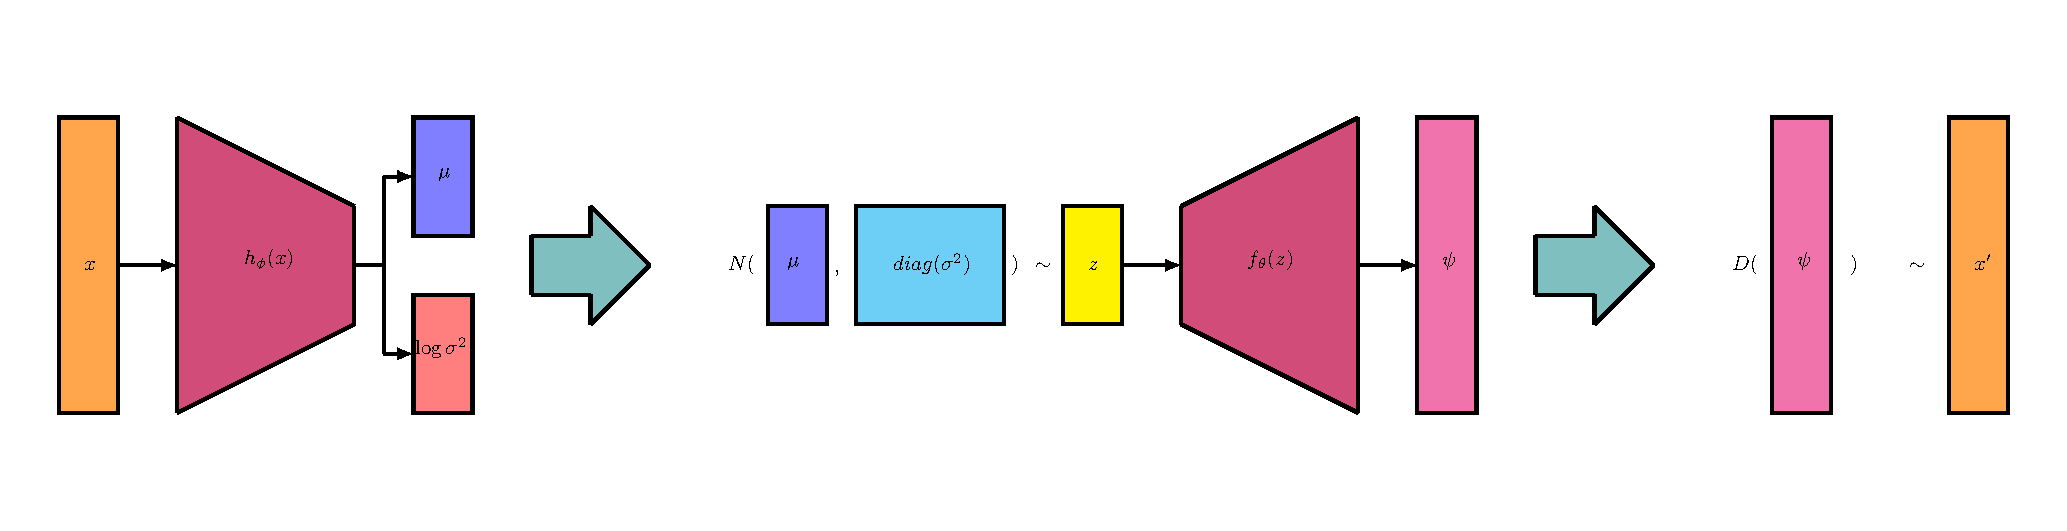
\includegraphics[width=12cm]{./TIKZ_TEX_FILE/PDFS/high_vae.pdf}};
        
            \begin{scope}[x={(image.south east)},y={(image.north west)}]
        
            
            \draw[red, thick] (0.83, 0.2) rectangle (0.98, 0.8);
            \draw[red, thick, fill, opacity=0.15] (0.83, 0.2) rectangle (0.98, 0.8);
            % \node[red, font=\small] at (0.3, 0.72) {Highlighted Area};
        
            \end{scope}
        \end{tikzpicture} 
    \end{center}

    \pause
    
    \begin{tcolorbox}[colback=blue!5!white, colframe=blue!75!black, fonttitle=\small, fontupper=\footnotesize]
    The \textbf{VAE} generates data \( \mathbf{x'} \) with the same input dimension as \( \mathbf{x} \) using the latent variable \( \mathbf{z} \), i.e., \( \mathbf{x'} \in \mathbb{R}^d \) where \( d \) is the input dimension.
    \end{tcolorbox}
\end{frame}

\begin{frame}{Key Techniques in VAE Construction}
    The construction of a \textbf{Variational Autoencoder (VAE)} is simple in structure, but utilizes several complex techniques to achieve its goal. These techniques include:

    \vspace{1em}
    
    \begin{tcolorbox}[colback=blue!5!white, colframe=blue!75!black, fonttitle=\small, fontupper=\footnotesize]
        \textbf{Reconstruction Loss}
    \end{tcolorbox}

    \pause
    
    \begin{tcolorbox}[colback=teal!5!white, colframe=teal!75!black, fonttitle=\small, fontupper=\footnotesize]
        \textbf{Kullback-Leibler (KL) Divergence}
    \end{tcolorbox}

    \pause
    
    \begin{tcolorbox}[colback=purple!5!white, colframe=purple!75!black, fonttitle=\small, fontupper=\footnotesize]
        \textbf{Evidence Lower Bound (ELBO)}
    \end{tcolorbox}

    \pause

    \begin{tcolorbox}[colback=orange!5!white, colframe=orange!75!black, fonttitle=\small, fontupper=\footnotesize]
        \textbf{The Reparameterization Trick}
    \end{tcolorbox}
\end{frame}

\begin{frame}{\textbf{Reconstruction Loss}}
    \begin{tcolorbox}[colback=red!20!white, colframe=red!70!black, title=\textbf{Reconstruction Loss}]
        Measures the difference between the input \( x \) and the reconstructed output \( \hat{x} \).
    \end{tcolorbox}

    \pause

    \begin{tcolorbox}[colback=teal!10!white, colframe=teal!70!black, title=\textbf{Common Metrics}]
        \begin{itemize}
            \item \textbf{Mean Squared Error (MSE)}:
                \[
                \mathcal{L}_{\text{recon}} = \| x - \hat{x} \|^2
                \]
            \item \textbf{Binary Cross-Entropy (BCE)} for binary data.
        \end{itemize}
    \end{tcolorbox}    
\end{frame}  

\begin{frame}{\textbf{Kullback-Leibler (KL) Divergence}}
    \begin{tcolorbox}[colback=blue!20!white, colframe=blue!70!black]
        Measures the divergence between \( q(z|x) \) and the prior \( p(z) \), typically \( \mathcal{N}(0, I) \).
    \end{tcolorbox}

    \pause

    \begin{tcolorbox}[colback=teal!10!white, colframe=teal!70!black, title=\textbf{Regularization Purpose}]
        Promotes a smooth, continuous latent space, fostering:
        \begin{itemize}
            \item \textbf{Continuity}
            \item \textbf{Completeness}
        \end{itemize}
    \end{tcolorbox}

    \pause
    
    \begin{tcolorbox}[colback=red!10!white, colframe=red!70!black, title=\textbf{KL Divergence Formula}]
        \[
        \mathcal{L}_{\text{KL}} = D_{\text{KL}}(q(z|x) \| p(z)) = \int q(z|x) \log \frac{q(z|x)}{p(z)} \, dz
        \]
    \end{tcolorbox}
\end{frame}

\begin{frame}{\textbf{Evidence Lower Bound (ELBO)}}
    \begin{tcolorbox}[colback=red!10!white, colframe=red!75!black, title=\textbf{ELBO: Overview}]
        ELBO optimizes both \textbf{Reconstruction Quality} (minimizing \( \mathcal{L}_{\text{recon}} \)) and \textbf{Latent Space Regularization} (minimizing \( \mathcal{L}_{\text{KL}} \)).
    \end{tcolorbox}
    
    \vspace{1em}

    \begin{tcolorbox}[colback=teal!10!white, colframe=teal!75!black, title=\textbf{Goal}]
        Maximize ELBO to minimize the total VAE loss: 
        \[
        \mathcal{L}_{\text{VAE}} = \mathcal{L}_{\text{recon}} + \mathcal{L}_{\text{KL}}.
        \]
    \end{tcolorbox}
\end{frame}

\begin{frame}{\textbf{ELBO : Impact Visualization}}
     \begin{figure}
        \centering
        \includegraphics[width=0.9\textwidth]{img/variational-autoencoder-distribution.png}  % Adjust path and figure size as needed
        \caption{Effect of KL Divergence on Latent Space Representation}
        \label{fig:KL_latent_space}
    \end{figure}
\end{frame}

\begin{frame}{\textbf{Reparameterization Trick}}
    \begin{tcolorbox}[colback=blue!10!white, colframe=blue!75!black]
        Enables backpropagation through stochastic sampling in latent space.
    \end{tcolorbox}
    
    \vspace{0.5em}

    \begin{tcolorbox}[colback=teal!10!white, colframe=teal!75!black, title=\textbf{Mathematical Expression}]
        \[
        z = \mu + \epsilon \cdot \sigma, \quad \epsilon \sim \mathcal{N}(0, I)
        \]
    \end{tcolorbox}
    
    \vspace{0.5em}

    \begin{tcolorbox}[colback=red!10!white, colframe=red!75!black, title=\textbf{Purpose}]
        Allows gradients to flow through \(\mu\) and \(\sigma\), bypassing non-differentiable sampling.
    \end{tcolorbox}
\end{frame}

\begin{frame}{Key Differences Between Autoencoder and Variational Autoencoder}

\begin{table}[ht]
\centering
\scriptsize % Slightly larger than tiny font size
\renewcommand{\arraystretch}{1.5} % Increases row height for better spacing
\begin{tabular}{|p{0.15\textwidth}|p{0.35\textwidth}|p{0.35\textwidth}|}
\hline
\rowcolor{blue!20} \textbf{Feature} & \textbf{Standard Autoencoder} & \textbf{Variational Autoencoder} \\ \hline

\textbf{Latent Space Representation} & Deterministic latent space. Each input maps to a single fixed latent vector. & \textbf{Probabilistic latent space.} Encodes inputs as distributions (mean \( \mu \) and variance \( \sigma^2 \)).\\ \hline 

\rowcolor{blue!10}\textbf{Loss Function} & Minimizes reconstruction error (e.g., MSE or cross-entropy). & Combines reconstruction loss with KL divergence,\(\mathcal{L} = \mathbb{E}_{q(z)}[\log p(x|z)] - \text{KL}(q(z) || p(z))\). \\ \hline 

\textbf{Generative Capability} & Non-generative: lacks a probabilistic model to sample data. & \textbf{Generative:} Samples latent vectors \( z \sim \mathcal{N}(\mu, \sigma^2) \) for new data generation. \\ \hline

\end{tabular}
\end{table}

\end{frame}

\begin{frame}{Key Differences Between Autoencoder and Variational Autoencoder}

\begin{table}[ht]
\centering
\scriptsize % Slightly larger than tiny font size
\renewcommand{\arraystretch}{1.5} % Increases row height for better spacing
\begin{tabular}{|p{0.15\textwidth}|p{0.35\textwidth}|p{0.35\textwidth}|}
\hline
\rowcolor{blue!20} \textbf{Feature} & \textbf{Standard Autoencoder} & \textbf{Variational Autoencoder} \\ \hline

\textbf{Regularization} & No explicit regularization on latent space. & Regularizes latent space to follow a prior (usually \( \mathcal{N}(0,1) \)). \\ \hline

\rowcolor{blue!10} \textbf{Philosophy} & Deterministic function mapping input to a compressed encoding and reconstruction. & Bayesian approach: learns a probabilistic model of data distribution \( p(x,z) \). \\ \hline

\textbf{Applications} & Compression, denoising, and feature extraction. & Generative modeling, anomaly detection, and latent space interpolation. \\ \hline
\end{tabular}
\end{table}

\end{frame}


\begin{frame}{Conditional Variational Autoencoder (CVAE)}

    % First Textbox: Limitations of Vanilla VAE
    \begin{center}
        \begin{tcolorbox}[colframe=red!50!black, colback=red!10!white, coltitle=black, sharp corners=south, boxrule=0.8mm, width=0.85\textwidth]
            \scriptsize
            \textbf{\textcolor{red}{Limitations of Vanilla VAE}}\\
            \vspace{0.2cm}
            One shortcoming of conventional \textbf{vanilla VAEs} is that the user has no control over the specific outputs generated by the autoencoder. For example, a conventional VAE trained on the MNIST dataset will generate new samples of handwritten digits from 0 to 9, but it cannot be constrained to output only \textbf{\textcolor{red}{4s}} and \textbf{\textcolor{red}{7s}}.
        \end{tcolorbox}
    \end{center}

    \pause
    \vspace{0.5cm}  % Add some space between the textboxes 
    
    % Second Textbox: Conditional VAE Advantage
    \begin{center}
        \begin{tcolorbox}[colframe=teal!50!black, colback=teal!10!white, coltitle=black, sharp corners=north, boxrule=0.8mm, width=0.85\textwidth]
            \scriptsize
            \textbf{\textcolor{teal}{Conditional VAE Advantage}}\\
            \vspace{0.2cm}
            \textbf{CVAEs} enable outputs conditioned on specific inputs, rather than solely generating variations at random. This is achieved by incorporating elements of \textbf{supervised learning} alongside the unsupervised objectives of conventional autoencoders, allowing for controlled generation based on labels or attributes.
        \end{tcolorbox}
    \end{center}
\end{frame}

\begin{frame}{CVAE v/s VAE}
    \begin{figure}
        \centering
        \includegraphics[width=0.7\linewidth]{img/cvae.png}
        \caption{Sample CVAE and VAE Architechture}
        \label{fig:enter-label}
    \end{figure}
    
\end{frame}
\begin{frame}{Generative Models Overview}

    % First Textbox: Generative Models Overview
    \begin{center}
        \begin{tcolorbox}[colframe=blue!50!black, colback=blue!10!white, coltitle=black, sharp corners=south, boxrule=0.8mm, width=0.85\textwidth]
            \scriptsize
            \textcolor{blue}{\textbf{Generative Models:}} \\
            Autoencoders like VAEs, CVAEs, and MADE are all examples of generative models. These models learn the underlying distribution of the data and are capable of generating new data points that resemble the original data.
        \end{tcolorbox}
    \end{center}

    \pause
    
    % Second Textbox: MADE Overview
    \begin{center}
        \begin{tcolorbox}[colframe=orange!50!black, colback=orange!10!white, coltitle=black, sharp corners=north, boxrule=0.8mm, width=0.85\textwidth]
            \scriptsize
            \textcolor{orange}{\textbf{MADE (Masked Autoencoder for Distribution Estimation):}} \\
            A generative model that utilizes \textcolor{purple}{\textbf{masking}} for distribution estimation.
        \end{tcolorbox}
    \end{center}

    \pause
    
    % Third Textbox: Key Aspects of MADE
    \begin{center}
        \begin{tcolorbox}[colframe=red!50!black, colback=red!10!white, coltitle=black, sharp corners=south, boxrule=0.8mm, width=0.85\textwidth]
            \scriptsize
            \textcolor{red!50}{\textbf{Key Aspects of MADE:}}
            \begin{itemize}
                \item \textcolor{black}{Masking Mechanism}
                \item \textcolor{black}{Generative Model}
                \item \textcolor{black}{Autoregressive Nature}
            \end{itemize}
        \end{tcolorbox}
    \end{center}
\end{frame}

\begin{frame}{Masked Autoencoder for Distribution Estimation}
    \begin{center}
        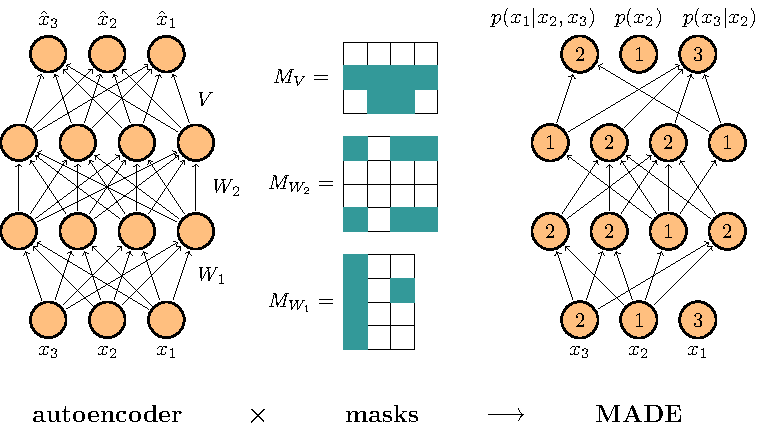
\includegraphics[width=0.75\textwidth]{./TIKZ_TEX_FILE/PDFS/made_pdf.pdf}  % Use your TikZ PDF file here
    \end{center}
\end{frame}

\begin{frame}[allowframebreaks]{References}
    \centering
    \scriptsize
    \begin{tcolorbox}[colframe=red!70!black, colback=red!10!white, coltitle=black, sharp corners=south, boxrule=0.8mm, width=0.85\textwidth, arc=4mm]
        \textbf{[1]} Kingma, D. P., \& Welling, M. (2013). Auto-Encoding Variational Bayes. \emph{International Conference on Learning Representations (ICLR)}.
    \end{tcolorbox}
    
   \begin{tcolorbox}[colframe=red!70!black, colback=red!10!white, coltitle=black, sharp corners=south, boxrule=0.8mm, width=0.85\textwidth, arc=4mm]
        \textbf{[2]} \href{https://www.ibm.com/think/topics/variational-autoencoder}{What is Variational Autoencoder?} by IBM.
    \end{tcolorbox}

    \begin{tcolorbox}[colframe=red!70!black, colback=red!10!white, coltitle=black, sharp corners=south, boxrule=0.8mm, width=0.85\textwidth, arc=4mm]
        \textbf{[3]} \href{https://mbernste.github.io/posts/vae/}{Variational Autoencoder} by Matthew N. Bernstein.
    \end{tcolorbox}

     \begin{tcolorbox}[colframe=red!70!black, colback=red!10!white, coltitle=black, sharp corners=south, boxrule=0.8mm, width=0.85\textwidth, arc=4mm]
        \textbf{[4]} \href{https://www.jeremyjordan.me/variational-autoencoders/}{Variational Autoencoder} by Jeremy Jordan.
    \end{tcolorbox}
\end{frame}



% FARIHA IFRAT - 2105059


\begin{frame}{\textbf{What is a Denoising Autoencoder?}}
    \vspace{1em}
    \begin{tcolorbox}[colback=teal!5, colframe=teal, title=\textbf{Definition}]
        A specialized \textbf{autoencoder} trained to reconstruct \textbf{clean data} from noisy inputs.
    \end{tcolorbox}
    \pause
    \vspace{1em}
    \begin{tcolorbox}[colback=yellow!10, colframe=yellow, title=\textbf{Key Goal}]
        \textbf{Remove noise} while preserving the \textbf{essential features} of the input.
    \end{tcolorbox}
\end{frame}

\begin{frame}{Summary}
     \vspace{1cm}
    \begin{block}{\textbf{Summary}}
        \centering
        A \textbf{denoising autoencoder} focuses on \textbf{eliminating noise from input data}, ensuring that important features are retained during the reconstruction process.
    \end{block}
    \vspace{1cm}
\end{frame}
\begin{frame}{What is a Denoising Autoencoder?}
\centering
   \begin{tikzpicture}[
    font=\sffamily,
    encoder/.style={trapezium, draw=blue!70, fill=blue!20, thick, minimum width=2cm, minimum height=1.2cm, rotate=270},
    decoder/.style={trapezium, draw=orange!70, fill=orange!20, thick, minimum width=2cm, minimum height=1.2cm, rotate=90},
    bottleneck/.style={rectangle, draw=purple!70, fill=purple!20, thick, minimum width=1.2cm, minimum height=1.2cm},
    arrow/.style={thick,->},
    image/.style={inner sep=0pt, anchor=center}
]

% Input Image
\node[image] (x) {\includegraphics[width=1.5cm]{Encoder/NoisyPic.png}};
\node[above=0.4cm of x, font=\small, align=center, text=blue!100] {\textbf{Input}};
\node[below=0.5cm of x, font=\small, text=blue!100] {$\mathbf{x}$};

% Encoder
\node[encoder, right=1.8cm of x] (encoder) {};
\node[above=0.4cm of encoder, font=\small, align=center, text=blue!100] {\textbf{Encoder }\\ $\mathbf{g_\phi}$};
\draw[arrow] (x) -- (encoder);

% Bottleneck
\node[bottleneck, right=1.8cm of encoder] (z) {$\mathbf{z}$};
\node[above=0.4cm of z, font=\small, align=center, text=purple!100] {\textbf{Bottleneck}};
\node[below=0.6cm of z, text width=3cm, align=center, font=\small, text=purple!70]{A compressed low \\ dimensional representation \\ of the input.};
\draw[arrow] (encoder) -- (z);

% Decoder
\node[decoder, right=1.8cm of z] (decoder) {};
\node[above=0.4cm of decoder, font=\small, align=center, text=orange!100] {\textbf{Decoder }\\ $\mathbf{f_\theta}$};
\draw[arrow] (z) -- (decoder);

% Reconstructed Image
\node[image, right=1.8cm of decoder] (x_prime) {\includegraphics[width=1.5cm]{Encoder/denoisedPic.png}};
\node[above=0.4cm of x_prime, font=\small, align=center, text=orange!70] {\textbf{Output}};
\node[below=0.5cm of x_prime, font=\small, text=orange!100] {$\mathbf{x'}$};
\draw[arrow] (decoder) -- (x_prime);

% Dashed line (ideally identical)
\node[above=0.3cm of x.east, xshift=4.5cm, font=\small, align=center, text=gray!70] {Ideally, they are identical: \\ $\mathbf{x} \approx \mathbf{x'}$};

\end{tikzpicture}
\end{frame}

% Slide 4: Architecture of a Denoising Autoencoder
% \begin{frame}{Architecture of a Denoising Autoencoder}
%     \begin{columns}
%         \column{0.5\textwidth}
%         \begin{itemize}[<+->]
%             \item Input: Noisy data.
%             \item Encoder:
%             \begin{itemize}
%                 \item Compresses noisy input into latent representation.
%             \end{itemize}
%             \item Decoder:
%             \begin{itemize}
%                 \item Reconstructs clean data.
%             \end{itemize}
%         \end{itemize}
%         \column{0.5\textwidth}
%         \includegraphics[width=\textwidth]{Encoder/The-overall-structure-of-a-denoising-autoencoder.png} % Replace with an architecture diagram.
%     \end{columns}
% \end{frame}
\begin{frame}{ Denoising Autoencoder Diagram}
\tikzstyle{startstop} = [rectangle, rounded corners, minimum width=3cm, minimum height=1cm, text centered, draw=black, fill=red!30,drop shadow]
\tikzstyle{process} = [rectangle, minimum width=3cm, minimum height=1cm, text centered, draw=black, fill=blue!30,drop shadow]
\tikzstyle{decision} = [diamond, minimum width=1.5cm, minimum height=0.5cm, text centered, draw=black, fill=green!30,drop shadow]
\tikzstyle{data} = [trapezium, trapezium left angle=70, trapezium right angle=110, minimum width=3cm, minimum height=1cm, text centered, draw=black, fill=orange!30,drop shadow]
\tikzstyle{arrow} = [thick,->,>=stealth]
\tikzstyle{connect} = [draw, thick, color=black, opacity=0.5]
\tikzset{
    neuron/.style={circle, draw=black, thick, minimum size=0.7cm, text centered, text=white, font=\small, fill=blue!70},
    encoder/.style={rectangle, draw=orange!60, thick, fill=orange!30, rounded corners, minimum width=2.5cm, text centered, font=\bfseries},
    decoder/.style={rectangle, draw=blue!60, thick, fill=blue!30, rounded corners, minimum width=2.5cm, text centered, font=\bfseries},
    noisy/.style={rectangle, draw=green!60, thick, fill=green!30, rounded corners, minimum width=2.5cm, text centered, font=\bfseries},
    output/.style={rectangle, draw=red!60, thick, fill=red!30, rounded corners, minimum width=2.5cm, text centered, font=\bfseries},
    arrow/.style={->, thick, >=stealth, draw=black!80},
    connect/.style={->, thick, draw=gray!80},
}


    \centering
    \scalebox{0.5}{
    \begin{tikzpicture}[x=2.5cm, y=1.5cm]

        % Labels
        \node[noisy] (input) at (0,0) {Noisy Input};
        \node[encoder] (encoder) at (2,0) {Encoder};
        \node[neuron, fill=purple!70] (bottleneck) at (4,0) {Bottleneck};
        \node[decoder] (decoder) at (6,0) {Decoder};
        \node[output] (reconstructed) at (8,0) {Reconstructed Output};

        % Layer Nodes
        \foreach \i in {1,...,6} {
            \node[neuron, fill=green!70] (input-\i) at (0, \i-3.5) {\i};
        }
        \foreach \i in {1,...,4} {
            \node[neuron, fill=orange!70] (encoder-\i) at (2, \i-2.5) {\i};
        }
        \foreach \i in {1,...,4} {
            \node[neuron, fill=blue!70] (decoder-\i) at (6, \i-2.5) {\i};
        }
        \foreach \i in {1,...,6} {
            \node[neuron, fill=red!70] (output-\i) at (8, \i-3.5) {\i};
        }

        % Connections
        \foreach \i in {1,...,6} {
            \foreach \j in {1,...,4} {
                \draw[connect] (input-\i) -- (encoder-\j);
            }
        }
        \foreach \i in {1,...,4} {
            \draw[connect] (encoder-\i) -- (bottleneck);
        }
        \foreach \i in {1,...,4} {
            \draw[connect] (bottleneck) -- (decoder-\i);
        }
        \foreach \i in {1,...,4} {
            \foreach \j in {1,...,6} {
                \draw[connect] (decoder-\i) -- (output-\j);
            }
        }

        % Annotations
        \node[above=0.5cm, align=center] at (encoder.north) {Feature Extraction};
        \node[above=0.5cm, align=center] at (decoder.north) {Feature Reconstruction};

    \end{tikzpicture}
    }
\end{frame}


% Slide 5: Mathematical Formulation
\begin{frame}{\textbf{Mathematical Formulation}}
    \begin{itemize}[<+->]
        \item \textbf{Given input \( x \)}, a noisy version \(\tilde{x}\) is created:
        \[\color{teal}
        \boldsymbol{\tilde{x} = x + \text{noise}}
        \]
        \item \textbf{Encoder maps \(\tilde{x}\)} to latent representation \( z \):
        \[\color{teal}
        \boldsymbol{z = f(\tilde{x}; \boldsymbol{\theta_e})}
        \]
        \item \textbf{Decoder reconstructs \(\hat{x}\)} from \( z \):
        \[\color{teal}
        \boldsymbol{\hat{x} = g(z; \boldsymbol{\theta_d})}
        \]
        \item \textbf{Loss function} minimizes reconstruction error:
        \[\color{teal}
        \boldsymbol{L(x, \hat{x}) = \|x - \hat{x}\|^2}
        \]
    \end{itemize}
\end{frame}



% Slide 6: Training a Denoising Autoencoder
\begin{frame}{\textbf{Training a Denoising Autoencoder}}
    \vspace{1em}
    \centering
    \scalebox{.7}{
    \centering
    \begin{tcolorbox}[colback=yellow!10, colframe=yellow!80, title=\textbf{Noise Addition}]
        \textbf{\color{teal}Types of Noise:}
        \begin{itemize}
            \item \textbf{Gaussian noise}
            \item \textbf{Salt-and-pepper noise}
        \end{itemize}
    \end{tcolorbox}
    }
    \vspace{1em}
    \pause
    
    \scalebox{.7}{
    \centering
    \begin{tcolorbox}[colback=cyan!10, colframe=cyan!70!black, title=\textbf{Objective}]
        \textbf{Minimize \color{red}reconstruction loss:}
        \[
        \boldsymbol{L(x, \hat{x}) = \|x - \hat{x}\|^2}
        \]
    \end{tcolorbox}
    }
    \vspace{1em}
    \pause
    
    \scalebox{.7}{
    \centering
    \begin{tcolorbox}[colback=blue!10, colframe=blue!70!black, title=\textbf{Optimization Techniques}]
        \textbf{\color{purple}Methods:}
        \begin{itemize}
            \item \textbf{Backpropagation}
            \item \textbf{Gradient Descent}
        \end{itemize}
    \end{tcolorbox}
    }
\end{frame}

\begin{frame}{Diagram}
\tikzstyle{startstop} = [rectangle, rounded corners, minimum width=3cm, minimum height=1cm, text centered, draw=black, fill=red!30,drop shadow]
\tikzstyle{process} = [rectangle, minimum width=3cm, minimum height=1cm, text centered, draw=black, fill=blue!30,drop shadow]
\tikzstyle{decision} = [diamond, minimum width=1.5cm, minimum height=0.5cm, text centered, draw=black, fill=green!30,drop shadow]
\tikzstyle{data} = [trapezium, trapezium left angle=70, trapezium right angle=110, minimum width=3cm, minimum height=1cm, text centered, draw=black, fill=orange!30,drop shadow]
\tikzstyle{arrow} = [thick,->,>=stealth]
\tikzstyle{connect} = [draw, thick, color=black, opacity=0.5]
\tikzset{
    neuron/.style={circle, draw=black, thick, minimum size=0.7cm, text centered, text=white, font=\small, fill=blue!70},
    encoder/.style={rectangle, draw=orange!60, thick, fill=orange!30, rounded corners, minimum width=2.5cm, text centered, font=\bfseries},
    decoder/.style={rectangle, draw=blue!60, thick, fill=blue!30, rounded corners, minimum width=2.5cm, text centered, font=\bfseries},
    noisy/.style={rectangle, draw=green!60, thick, fill=green!30, rounded corners, minimum width=2.5cm, text centered, font=\bfseries},
    output/.style={rectangle, draw=red!60, thick, fill=red!30, rounded corners, minimum width=2.5cm, text centered, font=\bfseries},
    arrow/.style={->, thick, >=stealth, draw=black!80},
    connect/.style={->, thick, draw=gray!80},
}


\centering
\scalebox{.7}{
\begin{tikzpicture}[node distance=3cm and 3cm]

% Nodes
% Arrows
\node (samples) [data] {Training Samples};

\pause
\node (corrupted) [process, below of=samples] {Corrupted Input};
\draw [arrow] (samples) -- (corrupted);

\pause
\node (hidden) [process, below of=corrupted] {Hidden Layers (Feature Vector)};
\draw [arrow] (corrupted) -- (hidden);

\pause
\node (reconstruction) [data, below of=hidden] {Reconstruction Signals};
\draw [arrow] (hidden) -- (reconstruction);

\pause
\node (error) [decision, right of=corrupted, xshift=3cm, text width=2.5cm] {Minimizing Reconstruction Error};
\draw [arrow] (corrupted.east) -- ++(0.5,0) |- (error.west);

\pause
\node (fine) [startstop, below of=error] {Fine-tuning Weights};
\draw [arrow] (error) -- (fine);
\draw [arrow] (fine.west) -- ++(-0.5,0) |- (hidden.east);

\end{tikzpicture}
}
\end{frame}


% Slide 7: Applications of Denoising Autoencoders
\begin{frame}{\textbf{Applications of Denoising Autoencoders}}
    \begin{minipage}[t]{0.35\textwidth}
        \centering
        \includegraphics[width=0.8\textwidth]{image-processing.png} % Add appropriate image for illustration
        \vspace{0.5em}
        \textbf{\color{teal}Image Denoising} \\
        
    \end{minipage} \hfill
    \pause
    \begin{minipage}[t]{0.35\textwidth}
        \centering
        \includegraphics[width=0.8\textwidth]{voice-recorder.png} % Add appropriate image for illustration
        \vspace{0.5em}
        \textbf{\color{teal}Speech Enhancement} \\
        
    \end{minipage}
    \pause
    \vspace{1em}
    \begin{minipage}[t]{0.35\textwidth}
        \centering
        \includegraphics[width=0.8\textwidth]{quality-control.png} % Add appropriate image for illustration
        \vspace{0.5em}
        \textbf{\color{teal}Anomaly Detection} \\
        
    \end{minipage} \hfill
    \pause
    \begin{minipage}[t]{0.35\textwidth}
        \centering
        \includegraphics[width=0.8\textwidth]{database-storage.png} % Add appropriate image for illustration
        \vspace{0.5em}
        \textbf{\color{teal}Data Preprocessing} \\
       
    \end{minipage}
\end{frame}



\begin{frame}{\textbf{Example: Image Denoising}}
    \begin{columns}
        % Left Column
        \column{0.4\textwidth}
        \vspace{1em}
        \begin{itemize}
            \item \textbf{Input:} Noisy images
            \item \textbf{Output:} Clean images
        \end{itemize}
        
        % Right Column
        \column{0.6\textwidth}
        \centering % Ensures the animation is centered in the column
        \scalebox{0.9}{
            \begin{animateinline}[autoplay,loop]{5} % Animation with 5 fps
                \multiframe{19}{i=1+1}{ % 19 frames, incrementing i from 1 to 19
                \scalebox{.75}{
                    \includegraphics[width=0.9\linewidth]{frames2/frame_\i.png} % Adjust width for proper scaling
                    }
                }
            \end{animateinline}
        }
    \end{columns}
\end{frame}


\begin{frame}{Example: Anomaly Detection}
\centering
\scalebox{.8}{
\begin{animateinline}[autoplay,loop]{10} % 10 fps animation
    \multiframe{19}{i=1+1}{ % 20 frames, incrementing i from 1 to 20
        \includegraphics[width=12cm]{frames/frame_\i.png} % Corrected file path
    }
\end{animateinline}
}
\end{frame}


% Slide 9:  Challenges
\begin{frame}{\textbf{Challenges of Denoising Autoencoders}}
    \begin{columns}[T] % Align top
        \column{0.5\textwidth}
        \centering
        \includegraphics[width=0.7\textwidth]{challenge2.jpg} % Replace with actual image
        \\[0.3cm]
        \textbf{\textcolor{teal}{Requires Diverse Noisy Data}}
        \pause
        \column{0.5\textwidth}
        \centering
        \includegraphics[width=0.7\textwidth]{challenge1.jpg} % Replace with actual image
        \\[0.3cm]
        \textbf{\textcolor{teal}{Sensitivity to Noise Types}} 
    \end{columns}
\end{frame}


% Slide 10: Conclusion
\begin{frame}{\textbf{Conclusion}}
    \vspace{1em}
    \begin{tcolorbox}[colback=teal!10, colframe=teal, boxrule=0.5mm, rounded corners]
        \centering
        \textbf{\textcolor{teal!80!black}{Autoencoders: Driving Smarter Data Innovations}}
    \end{tcolorbox}
    
    \vspace{1em}
    \pause
    \begin{columns}[T]
        \column{0.5\textwidth}
        \begin{tcolorbox}[colback=blue!10, colframe=blue!60, boxrule=0.3mm, rounded corners]
            \textbf{\textcolor{blue!70!black}{\large Fundamentals}}\\
            Mastering key concepts for smarter systems.
        \end{tcolorbox}
        
        \vspace{1em}
        \pause
        \begin{tcolorbox}[colback=purple!10, colframe=purple!60, boxrule=0.3mm, rounded corners]
            \textbf{\textcolor{purple!70!black}{\large Versatility}}\\
            Adapts seamlessly to diverse applications.
        \end{tcolorbox}
        \pause
        \column{0.5\textwidth}
        \begin{tcolorbox}[colback=green!10, colframe=green!60, boxrule=0.3mm, rounded corners]
            \textbf{\textcolor{green!70!black}{\large Impact}}\\
            Enhancing data quality and feature discovery.
        \end{tcolorbox}
        \pause
        \vspace{1em}
        
        \begin{tcolorbox}[colback=orange!10, colframe=orange!60, boxrule=0.3mm, rounded corners]
            \textbf{\textcolor{orange!70!black}{\large Future}}\\
            Unlocking endless AI opportunities.
        \end{tcolorbox}
    \end{columns}
\end{frame}


\begin{frame}{\textbf{Thank You!}}
\centering
\includegraphics[width=0.6\textwidth]{teachers-day.png} 
    
\end{frame}


\end{document}